\documentclass[conference]{IEEEtran}
\usepackage{cite}
\usepackage{pdfpages}
\usepackage[utf8]{inputenc}
\usepackage{amsmath,amssymb,amsfonts}
\usepackage{algorithmic}
\usepackage{graphicx}
\usepackage{textcomp}
\usepackage{xcolor}
\usepackage{tabularx}
\usepackage{colortbl}
\usepackage{multirow}
\usepackage{multicol}
\usepackage[export]{adjustbox}
\def\BibTeX{{\rm B\kern-.05em{\sc i\kern-.025em b}\kern-.08em
    T\kern-.1667em\lower.7ex\hbox{E}\kern-.125emX}}
\begin{document}

\title{\textsc{
    Projektrapport\\
    II1302 Projekt och projektmetoder, grupp 8\\
{\large Förslag på en fungerande projektmetod för små IT-projekt}}

% To accommodate for the .doc's formatting, the author blocks have been replaced with this section instead.
\begin{center}
    \large{ 
        Abyel Tesfay\textsuperscript{1}, Adam Liliemark\textsuperscript{2}, 
        Alexander Jonsson\textsuperscript{3}, Elias Johansson\textsuperscript{4}, 
        Mikael Andersson\textsuperscript{5}\\
        \textit{\\School of Electrical Engineering and Computer Science\\
                KTH Royal Institute of Technology\\
                SE-100 44 Stockholm, Sweden\\}
        \textsuperscript{1}\texttt{abyel@kth.se}\\
        \textsuperscript{2}\texttt{adamlil@kth.se}\\
        \textsuperscript{3}\texttt{alexjons@kth.se}\\
        \textsuperscript{4}\texttt{eliajo@kth.se}\\
        \textsuperscript{5}\texttt{mian3@kth.se}
    }
\end{center}
}

% This is just to kill the warning about no author given.
\author{}

\maketitle

% Mikael
\begin{abstract}
Utifrån en given startmetod med hjälp av flera olika litteraturkällor tillsammans med att helt enkelt pröva sig fram har gruppen försökt att hitta en väl fungerande metod för att så effektivt och produktivt som möjligt utveckla små IT-projekt. Genom att kontinuerligt diskutera metoden under arbetets gång har flera modifieringar kunnat genomföras och på så sätt har en anpassad metod kunnat långsamt växa fram. Även om små grupper i små projekt ofta gärna bildar ett mer dynamiskt arbetssätt och att det därmed kan vara svårt att finna en generell modell så har gruppen lyckats hitta en metod som fungerade väldigt bra för just denna gruppen i detta projektet. Även om resultatet inte har ett helt entydigt resultat så uppfyller det likväl både kursens syfte och mål eftersom den ursprungliga undersökningsfrågan faktiskt besvaras.
\end{abstract}

\begin{IEEEkeywords}
IoT, JavaScript, React, Firebase, Google Cloud, Personsökare, Pager, Connected devices, Projektmodell, Projektmetod, SCRUM, IT-projekt, II1302
\end{IEEEkeywords}

% Abyel
\section{Om detta dokument och undersökning}
Följande dokument riktar sig till studenter, examinatorer och övriga deltagare till kursen \textit{II1302 Projekt och Projektmetoder} men kan studeras av läsare med en position inom akademi 
eller IT-företag. Dokumentet delas in i ett antal kapitel där de första beskriver kursens bakgrund och problemformulering, samt de krav som studenterna förväntas uppfylla via denna rapport.
Rapporten är en teoristudie innehållande en litteratur- och förstudie som används till grund för undersökningen, samt en beskrivning på den undersökningsmetod som använts och hur den 
uppfyller kraven för vetenskapligt arbetssätt. De senare kapitlen redovisar genomförandet av projektarbetet utifrån de metoder, praxis och 
verktyg som använts, resultat av utfört projektarbete samt en analys och diskussion om hur problemformuleringen kan lösas med en slutsats som grundar sig på utförd teoristudie och resultat utav projektarbetet.

Då större fokus lagts i kursens projektarbete och att projektarbete kan ge olika resultat utifrån faktorer såsom gruppdynamik, omfattning 
och gruppmedlemmars tillgänglighet kan rapportens trovärdighet ifrågasättas. Alla deltagande studenter inom kursen har däremot utfört liknande 
projektarbeten med fokus på IT (webbdesign, mjuk- och hårdvara samt nätverk) och med samma förvalda projektmetod utav kursen. Rapporten bör därav ha en genuin trovärdighet.

Projektets resultat d.v.s \textit{resultatmål} blev en webbapplikation som kommunicerar med en eller flera \textit{pagers}, enheter 
som kan hämta meddelanden som skickas från applikationen (se figur \ref{fig:webbapp} och \ref{fig:personsokare}). Kommunikationen mellan produkterna sker via en extern databas
som förses av en molntjänst utav Google. Användaren skickar meddelanden från webbapplikationen till personsökare via en databas, dessa meddelanden hämtas sedan av personsökaren.\\

% Alex
\section{Introduktion}
Detta kapitel är avsett för att ge läsaren bakgrund till arbetet, där bakgrund innebär nödvändig information om kursen, 
vad som examineras och vad som skall förväntas av studenter i projektgruppen efter godkänd kurs.
Läsaren skall även få reda på kursens problemformulering, vilken/vilka strategier som använts samt avgränsningar.

\begin{figure}[h!]
    \centerline{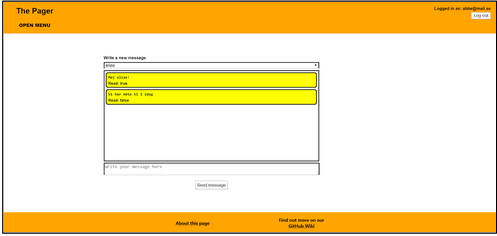
\includegraphics[max height=250px, max width=250px]{images/webbapplikation.png}}
    \caption{webbapplikation, \textit{gränssnitt}}
    \label{fig:webbapp}
\end{figure}

\begin{figure}[h!tbp]
    \centerline{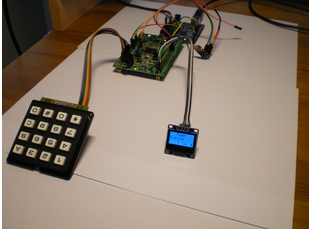
\includegraphics[max height=250px, max width=250px]{images/personsokare.png}}
    \caption{personsökare, hårdvara}
    \label{fig:personsokare}
\end{figure}

% Alex
\subsection{Bakgrund}\label{Bakgrund}
Kursen \textit{II1302 Projekt och projektmetoder} har som fokus att lära studenten, på ett sätt som är ansedd av vara praktiskt, om projektmetoder som kan användas inom IT-projekt. 
Studenter som tar denna kurs blir indelade i projektgrupper mellan 4–8 deltagare där deltagarna skall utföra någon form av IT-projekt, detta IT-projekt ska omfatta mjukvara, hårdvara, elektronik och nätverk.
Utifrån den givna projektmodellen skall idéer och diskussion för förändringar, som anpassar till olika typer av projekt, skapas.
Kursen har som huvudsaklig undersökningsfråga \textit{Vad är en bra projektmetod för små IT-projekt?} som skall besvaras av studenterna i projektgruppen i slutet av kursen i form av en gemensam rapport.
Kursen har inga särskilda behörigheter.\\
Efter studenten blivit godkänd ska den, "för små IT-projekt", kunna:
\begin{itemize}
    \item Föreslå och redogöra för en anpassad, användbar och beprövad projektmetod
    \item Utifrån någon ansvarsroll kunna ange, med evidens, motivera metoders styrkor och svagheter i koppling till det genomförda projektet
    \item Bidra till systemutvecklingsarbete samt idéer kring systemet
    \item Utifrån någon ansvarsroll planera, organisera, leda och veta hur projektgruppen ligger till med arbetet
    \item Engagera sig socialt, vara uppmuntrande och ansvarsfull till projektgruppen
    \item Förhålla sig till målsättningar som är ansedda att vara samhälleliga, t.ex. hållbarhet
\end{itemize}
Kursen examineras på tre olika sätt:
\begin{itemize}
    \item PRJ1 - Individuella dokument, 3,5 HP\\Betygsskala: A, B, C, D, E, FX, F
    \item RAP1 - Gruppgemensam rapport, 3,0 HP\\Betygsskala: A, B, C, D, E, FX, F
    \item UTV1 - Utvärderingsdokument, 1,0 HP\\Betygsskala: P, F
\end{itemize}
Kursens examinator är:
\begin{itemize}
    \item Anders Sjögren, \texttt{as@kth.se}
\end{itemize}
Projektet delades upp från start i fem iterationer av examinatorn där det tydligt sades vad som skall vara uppnått vid varje iteration.\\

% Adam
\subsection{Problemformulering}
Den övergripande frågeställningen i denna rapport är \textit{Vad är en bra projektmetod för små IT-projekt?}. Denna korta men tydliga fråga rymmer hela spektrumet från
hur individer ska arbeta individuellt till hur gruppen som enhet ska utvärdera det arbete som genomförts. För att svara på frågan delas den upp i mindre delar:
\begin{itemize}
    \item Hur ska gruppen rent konkret arbeta?
    \item På vilket sätt ska individer redovisa och samverka kring utfört arbete?
    \item Vem eller vilka ansvarar för att det logistiska, det vill säga arbete ej relaterat till produkten, genomförs?
    \item Hur ska arbetet, produkten och metoden utvärderas?
\end{itemize}

% Alex
\subsection{Undersökningsstrategi/lösningsstrategi}
Under kursens gång har kursmaterial och kurslitteratur tilldelats av kursens examinator i form av artiklar, kompendium, rapporter, böcker och mm. för studenter att 
läsa. Majoriteten av kursmaterialet var frivilligt att läsa, däremot så var en viss del av kursmaterialet (och litteratur) kopplat till inlämningsuppgifter och 
quizer som gavs till studenter under kursens gång. Detta tvingade studenter att faktiskt ta del av kursmaterialet och få en bättre förståelse över olika 
projektmetoder samt projektmodeller. Material har även presenterats under föreläsningar där olika projektmetoder samt utvecklingsmetoder har framställts för olika 
områden inom IT-projekt. Detta material har projektgruppen diskuterat under retrospektiva SCRUM-möten där projektgruppen har tittat på olika modeller samt metoder 
för att jämföra dem med det som användes under den tiden. Sedan har det tagits beslut om en eller flera förändringar bör ske eller ej. Den huvudsakliga 
frågeställningen för beslut om förslag för förändring har varit \textit{Underlättar denna förändring vårt kollektiva arbete kring IT-projektet?}

IT-projektets uppgift löstes genom iterativt arbete på både mjukvara och hårdvara under iteration ett, två, tre och fyra med dagliga SCRUM-möten för att uppdatera 
andra medlemmar i projektgruppen hur man ligger till i arbetet. IT-projektet adopterade tidigt en DevOps-kultur för  integration och utveckling av produkten samt 
system tillhörande till produkten.

Projektmedlemmar har tillsammans tagit eget ansvar för att se till att dokument och systemdokumentationer skrivits och blivit färdigställda innan sagd deadline.
Tillsammans har alla projektmedlemmar sett till att arbete har delats upp i rättvisa mängder.

% Adam
\subsection{Relaterade arbeten}
Alla studenter i gruppen har genomfört kursen \textit{II1300 Ingenjörsmetodik} och blivit godkända, där skrevs en rapport likt denna. II1300 bygger på samma 
grundtanke som denna kurs men är på en mer grundlig nivå som kan anses vara enklare, då det är en av de första kurserna högskoleingenjörsstudenter i Kista tar. Rapporten i II1300 är emellertid ett relevant relaterat arbete, där studenterna reflekterade över olika projektmetoder och testade dessa i praktiken.

De flesta gruppmedlemmarna använde under II1300 en scruminspirerad projektmetod, vilket även var fallet i denna kurs. 

Ytterligare ett relaterat arbete är Henrik Knibergs \textit{Scrum and XP From The Trenches}\cite{kniberg_scrum_2015}, där erfarenheter från att arbeta scrumbaserat tas upp.
Denna bok har varit en inspiration både vid skrivandet av denna rapport och under arbetet med projektuppgiften.

% Adam
\subsection{Avgränsningar}
Denna rapport behandlar i huvudsak scrum och den projektmetodik vi valt att använda. Övriga projektmetoder, så som XP, kommer ej behandlas.
Projektuppgiften i denna kurs är av liten omfattning, varför en avgränsning görs där; stora projekt som löper under längre tidsperiod än några månader är utanför denna
kurs och rapports omfattning.

% Micke
\section{Teori och ingenjörspraxis}
I detta kapitel beskrivs den litteratur som användes i kursen för att på  vetenskapligt och med evidens styrkta metoder prova oss fram i undersökningen. I mitten av kapitlet så redovisas gruppens olika rollkompetenser enligt Essence. I slutet av kapitlet beskrivs en del av ansatsen till den metod som gruppen tilldelades för att snabbt komma igång. Del av ansatsen är rollindelningen inför projektet.

% Micke
\subsection{Litteraturstudie}
Till denna rapport, samt fortlöpande under projektets gång, har olika källor använts för att få en breddad bild om olika projektmetoders styrka och svagheter. Litteraturen har lästs, helt eller delvis, som deluppgifter vid varje iteration. I vissa fall skapade studenterna egna instuderingsfrågor åt varandra.

\textbf{Litteraturkällor som använts:}
\begin{itemize}
    \item Kernel and Language for Software Engineering Methods (Essence 1.0) \cite{object_management_group_kernel_2014}
    \item Kniberg, H. Scrum from the trenches \cite{kniberg_scrum_2015}
    \item Eklund, S.  Arbeta i projekt: individen, gruppen, ledaren. \cite{Eklund:2} 
    \item Katter, A. (2015). Förslag till en ekonomiskt hållbar projektmetod. \cite{Katter}
    \item Introduction to Agile Project Management \cite{IntroAgileProjMan}
    \item Survey of Agile Tool Usage and Needs (Azizyan, Magarian, Kajko-Mattsson) \cite{SurveyofAgileTool}
    \item Alpha State Cards: Reference Guide (Jacobson, 2013) \cite{AlphaStateCard}
    \item Jacobson, Spence, Seidewitz, (2016). Industrial-Scale Agile. \cite{IndustrialScaleAgile}
    \item Kniberg, H. Skarin, M. (2009). Kanban and Scrum - Making the Most of Both \cite{KanbanandScrum}
\end{itemize}

\subsection{Kompetenser i gruppen}
Varje person i projektgruppen har ett ansvarsområde. Detta ansvarsområde innebär att respektive gruppmedlem kan utforma vår arbetsmetod genom att förändra och förbättra vårt sätt att arbeta. Vissa av dessa förändringar kan vara synliga på arbetstavlan, medan andra förändringar verkar i bakgrunden. I praktiken arbetade medlemmarna i gruppen tvärsektoriellt och hjälpte varandra inom respektives ansvarsområde.
De ansvarsområden, respektive kompetenser som fanns i gruppen var:

\textbf{Kund- och kravansvarig}

Besitter kompetens att sammanställa, kommunicera och balansera andra aktörers behov samt att representera dessa \cite{object_management_group_kernel_2014}.

Ansvarar för följande delar: 
\begin{itemize}
    \item Visionsdokument
    \item Kravdokument
    \item Stories / UseCase / UseCaseSlices
\end{itemize}


\textbf{Arkitektansvarig} 

Har kompetens att se och förstå systemmöjligheter och de behov som andra aktörer har, samt förmåga att översätta detta till förståeliga direktiv \cite{object_management_group_kernel_2014}.

Ansvarar för följande delar:
\begin{itemize}
    \item Arkitekturdiagram
\end{itemize}


\textbf{Utvecklingsansvarig}

Bemästrar kompetens att designa och programmera funktionella mjukvarusystem som följer riktlinjerna som gruppen överenskommit \cite{object_management_group_kernel_2014}.

Ansvarar för följande delar:
\begin{itemize}
    \item Design -och utvecklingsplan 
\end{itemize}


\textbf{Testansvarig}

Denna person besitter spetskompetens att testa ett system samt verifiera att systemet är användbart och att det lever upp till de ställda kraven \cite{object_management_group_kernel_2014}.

Ansvarar för följande delar:  
\begin{itemize}
    \item Teststrategi
    \item Testplan
    \item Testverktyg
\end{itemize}


\textbf{Projektledare}

Projektledaren är specialist på att inspirera och motivera gruppen att nå uppsatta mål. Att koordinera, planera och följa upp arbetet är också projektledarens uppgift \cite{object_management_group_kernel_2014}.

Ansvarar för följande delar: 
\begin{itemize}
    \item Projektplanering
    \item Projektdefinition
\end{itemize}


\textbf{Miljö, hållbar utveckling, etik, arbetsmiljö och jämställdhet}

Detta ansvarsområde delades inom gruppen. Ingen person tilldelades detta ansvarsområde. Det betyder inte att detta område är mindre viktigt, snarare tvärtom.

% Alex
\subsection{Förstudie}
Vid start av kurs tilldelades en metodansats av kursens examinator. Denna ansats innebar en iterativ metod där varje iteration hade en längd på två veckor (inkl. en 
extra iteration över påsk som var en vecka för eget arbete.) Denna metodansats verkade vara skapad utifrån SCRUM i baktanke och projektgruppen tog stor användning av detta. 
Dock så förekom vissa ändringar redan vid start av kurs som, enligt gruppen, känts lämpliga. 
SCRUM har tre huvudroller: 
\begin{itemize}
    \item Product owner (produktägare)\\
    \textit{Hanterar krav och önskemål om tillägg för produkten, tar även emot förändringsförslag}.
    \item Scrum master (scrummästare)\\
    \textit{Säkerställer efterlevnad av processen, ser till att alla aktörer är} up-to-date\textit{. Ser till att förhindra förekommandet av hinder för utvecklingsteamet. Kan även ses som} coach.
    \item Development team (utvecklingsteam)\\
    \textit{Självorganiserad grupp som utvecklar produkten i fråga}.
\end{itemize}

Projektgruppen har själva känt att de själva är ägaren av produkten, därav ingen enskild person med roll produktägare, 
en liknande roll som däremot har använts är kravansvarig. Projektgruppen har inte haft en scrummästare utan har tillsammans 
coachat varandra och vid varje SCRUM-möte sett till att uppdatera varandra med hur arbete ligger till. 
Alla i projektgruppen har utvecklat någon del av systemet, vilket innebär att alla medlemmar är en del av utvecklingsteamet. 
Dessa ändringar kan ses som de mest anmärkningsvärda då resterande byggstenar i SCRUM har mer eller mindre tagits del av.\\

\subsubsection{\textit{Arbetstavla (projektgruppens metodansats)}}
Det är viktigt att notera att på grund av den rådande pandemin (COVID-19) under denna tid har gjort att arbete enbart utförts \textit{online}, dvs. enbart distansstudier har utförts. 
Detta har inneburit att projektgruppens arbetstavla har befunnit sig \textit{online} med hjälp av verktyget Lucidchart.

Projektgruppens arbetstavla består av två sidor, en publik sida och en privat sida. På den publika sidan så finner man länkar till projektgruppens 
Projektdefinition, Visionsdokument, Gantt-schema och Kravdokument. Det finns även en länk till kursens betygskriterier. Stories och Use-Case models för 
kursrapporten samt själva produkten finns också på den publika sidan. Produktens Use-Cases har färgkodats för att skapa en bättre överblick som 
snabbt går att förstå, användandet och uppdelningen av färger har gjort det lättare att hitta och ta ut Use-Case slices. Dessa Use-Case slices gömmer 
sig under varje \textit{bubbla} som går att läsa om man så vill genom att klicka på dem. Se figur \ref{fig:ArbetstavlaPublik} för en bild på projektgruppens publika sida av arbetstavlan.

På den privata sidan av arbetstavlan så finner man projektgruppens burndown chart, bild på systemets arkitektur, projektgruppens nuvarande arbeten samt ett par 
listor. De listor som fanns behandlade risker, tester och oplanerade händelser. Viktigt att veta om projektgruppens burndown chart är att den inte är räknad i timmar 
utan är räknad i antalet arbetsuppgifter. Arbetsuppgifter fanns på arbetstavlan som post-it-lappar där det stod vad varje person har planerat att göra denna 
iteration. För att veta vems post-it-lapp som var vems så hade varje gruppmedlem blivit tilldelad en färg, la man till en arbetsuppgift såg man till att man satte 
sin färg på denna post-it-lapp. Under kursens gång så utvecklades denna idé och en liten ruta på post-it-lappen lades till i det övre högra hörnet, denna ruta skulle 
färgas beroende på vilken Use-Case som arbetsuppgiften tillhörde. Alla arbetsuppgifter sågs till att inte vara för stora eller för små, storleken av varje 
arbetsuppgift skulle bäst förklaras som \textit{lagom}. Se figur \ref{fig:ArbetstavlaPrivat} för en bild på projektgruppens privata sida av arbetstavlan.

\subsubsection{\textit{Scruminspirerade aktiviteter}}
Gruppen provade att utarbeta ett arbetssätt som passade förutsättningarna (distansstudier, små IT-projekt etc.) Projektgruppens arbetsstruktur såg ut på följande sätt för varje 
iteration:
\begin{itemize}
    \item \textbf{Iterationsplanering}
    \begin{enumerate}
        \item Iterationsmål\\
        \textit{Projektgruppen tittade på de mål som ska uppfyllas för iterationen.}
        \item Arbetstavla\\
        \textit{Arbetstavlan uppdaterade med nya arbetsuppgifter.}
        \item Use-Case slices\\
        \textit{Projektgruppen tittade på Use-Case slices för att finna ytterligare arbetsuppgifter i samband med dem.}
    \end{enumerate}
    \item \textbf{Dagligt arbete}\\
        \textit{Varje dag börjades med ett stand-up möte. Sedan gick projektgruppen över till dagligt projektarbete.}
    \item \textbf{Sprint demo}\\
    \textit{Varje iteration avslutades med en sprint demo.}
    \item \textbf{Retrospektivt möte om iterationen}\\
    \textit{Som sista möte så hölls ett retrospektivt möte där projektgruppen tittade på vad som gick bra och vad som kunde förbättras.}
\end{itemize}
Figur \ref{fig:DiagramArbetsstruktur} visar gruppens egna övergripande arbetssätt i ett diagramformat.

Färdiga arbetsmetodförslag finns som inspirerade projektgruppen i deras egna undersökande sätt att finna en bra projektmetod för små IT-projekt. Se figur \ref{fig:ivar} för 
en metodöversikt enligt Essence.

% Bilder som tillhör "Förstudie"
\begin{figure}[htbp]
    \centerline{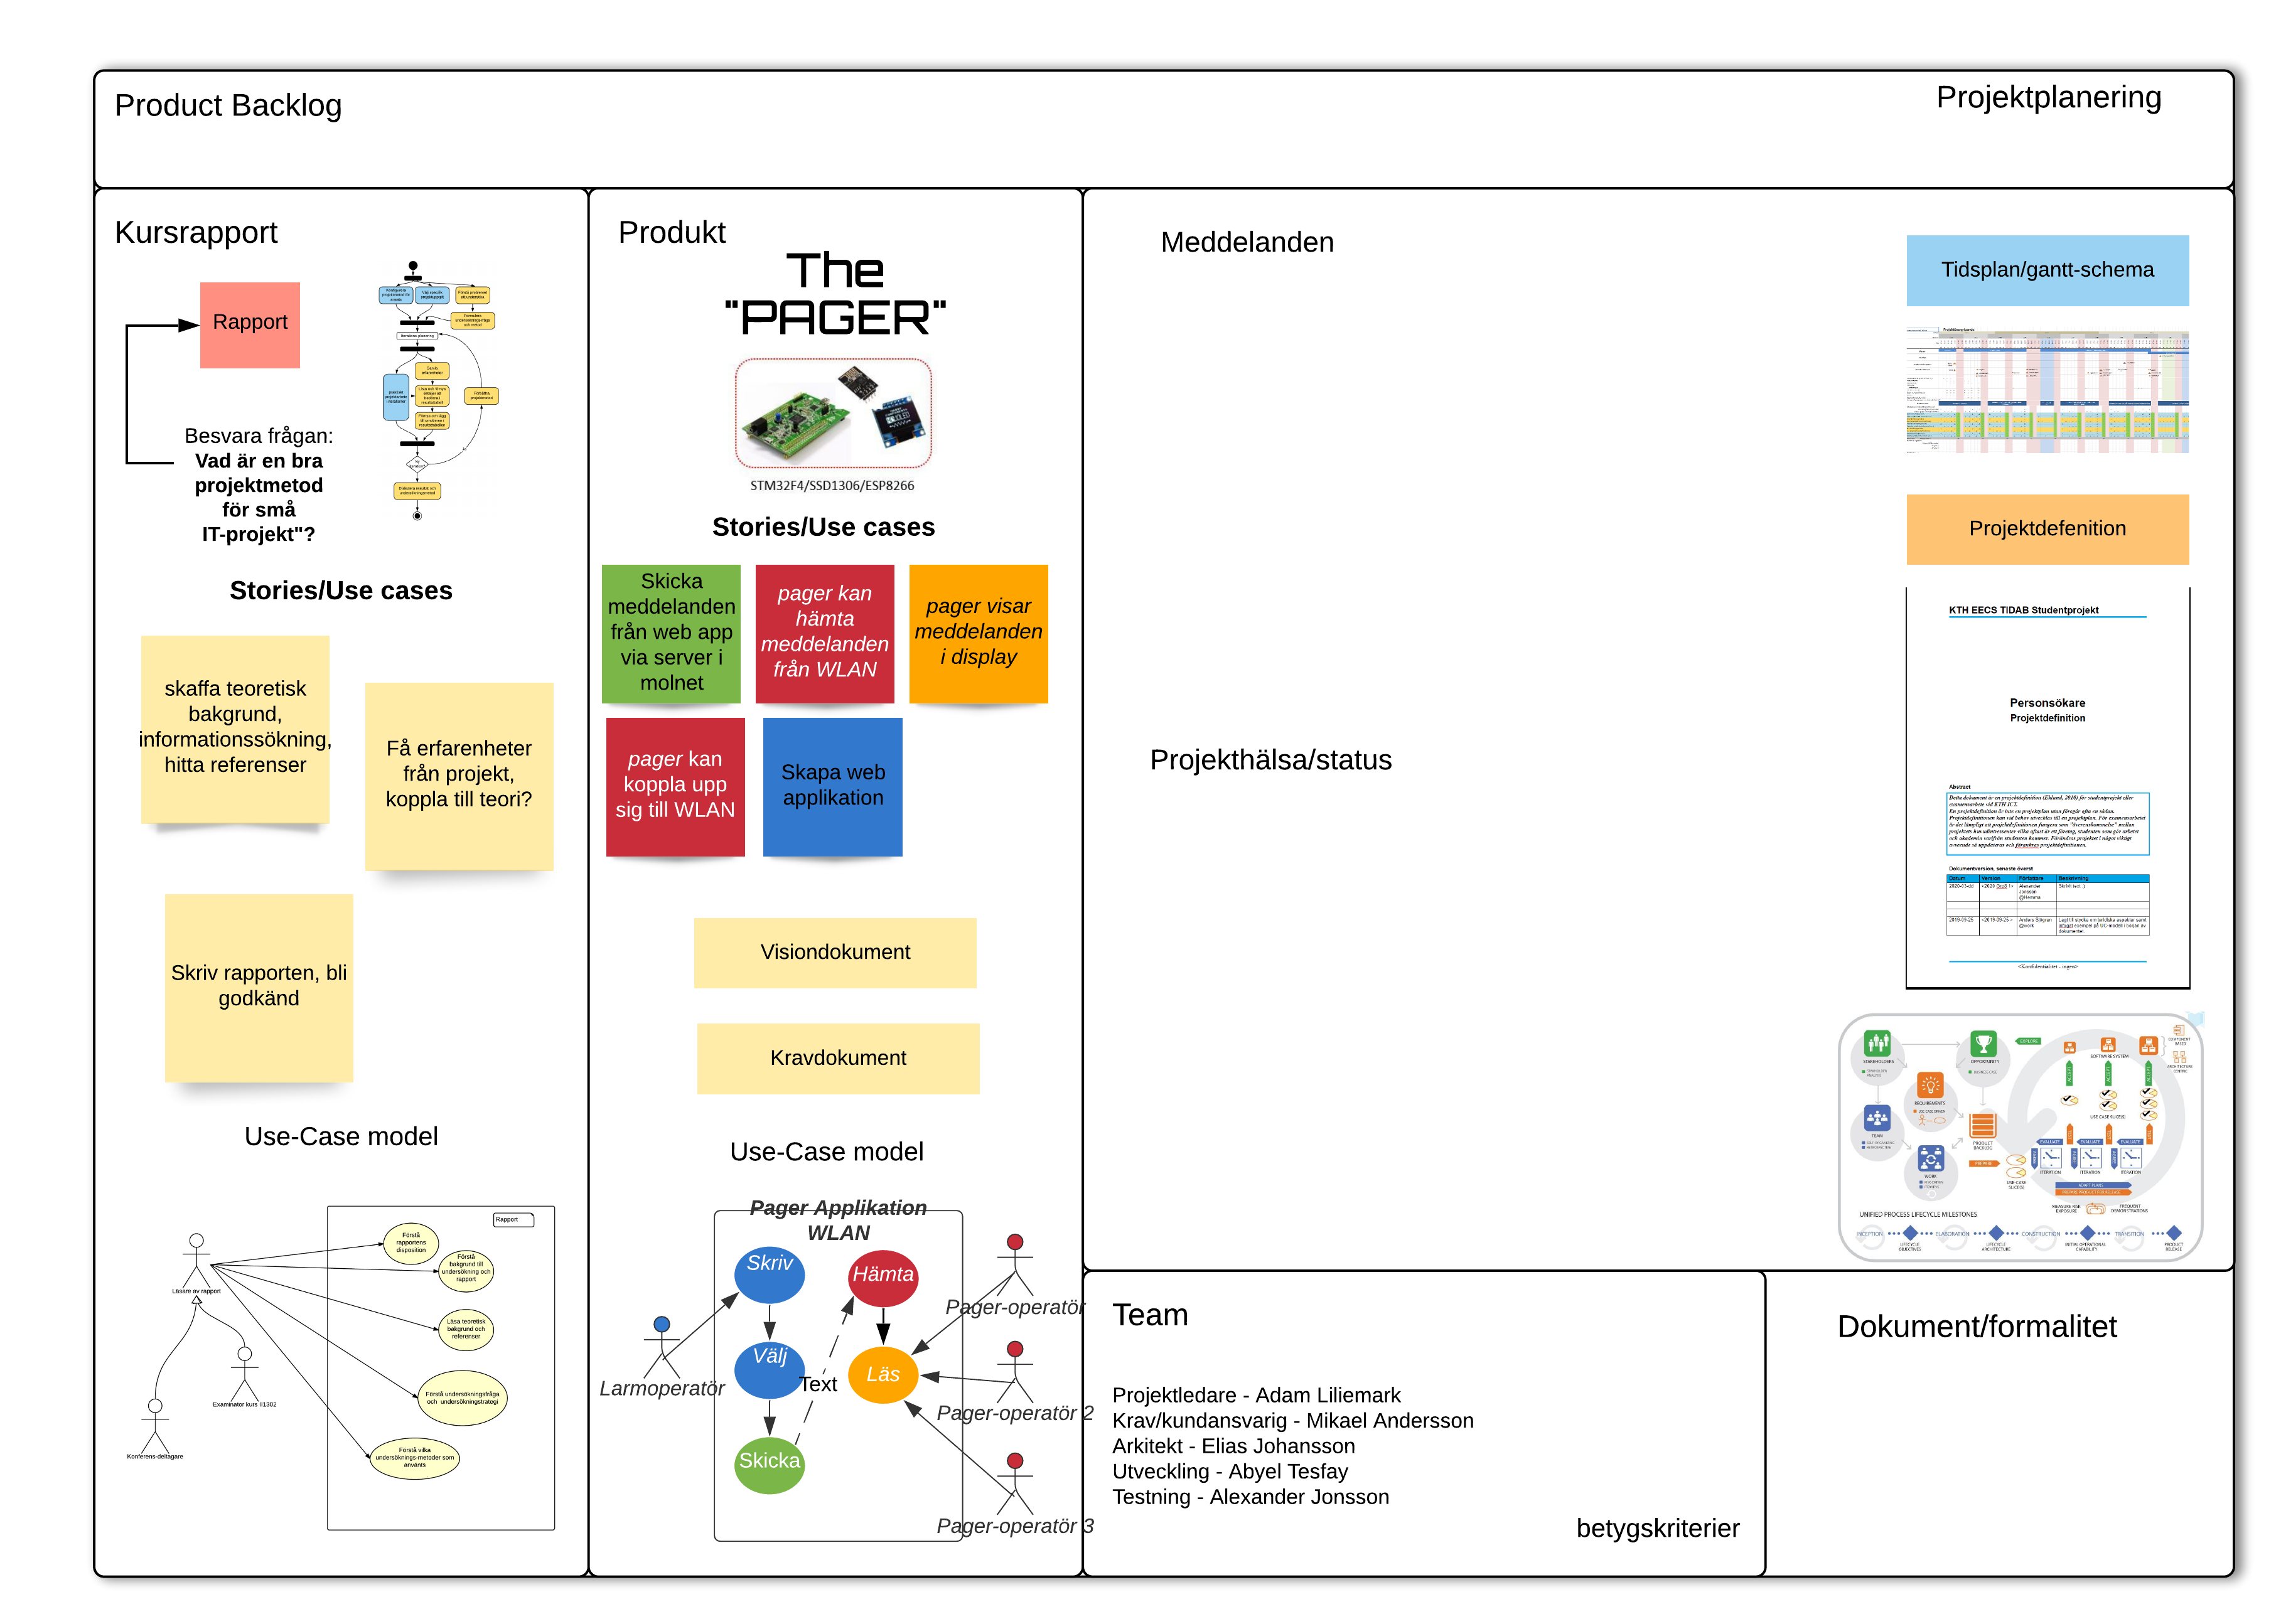
\includegraphics[max height=250px, max width=250px]{images/ArbetstavlaPublik.png}}
    \caption{Arbetstavla, \textit{whiteboard}, \textit{Publik sida}}
    \label{fig:ArbetstavlaPublik}
\end{figure}

\begin{figure}[htbp]
    \centerline{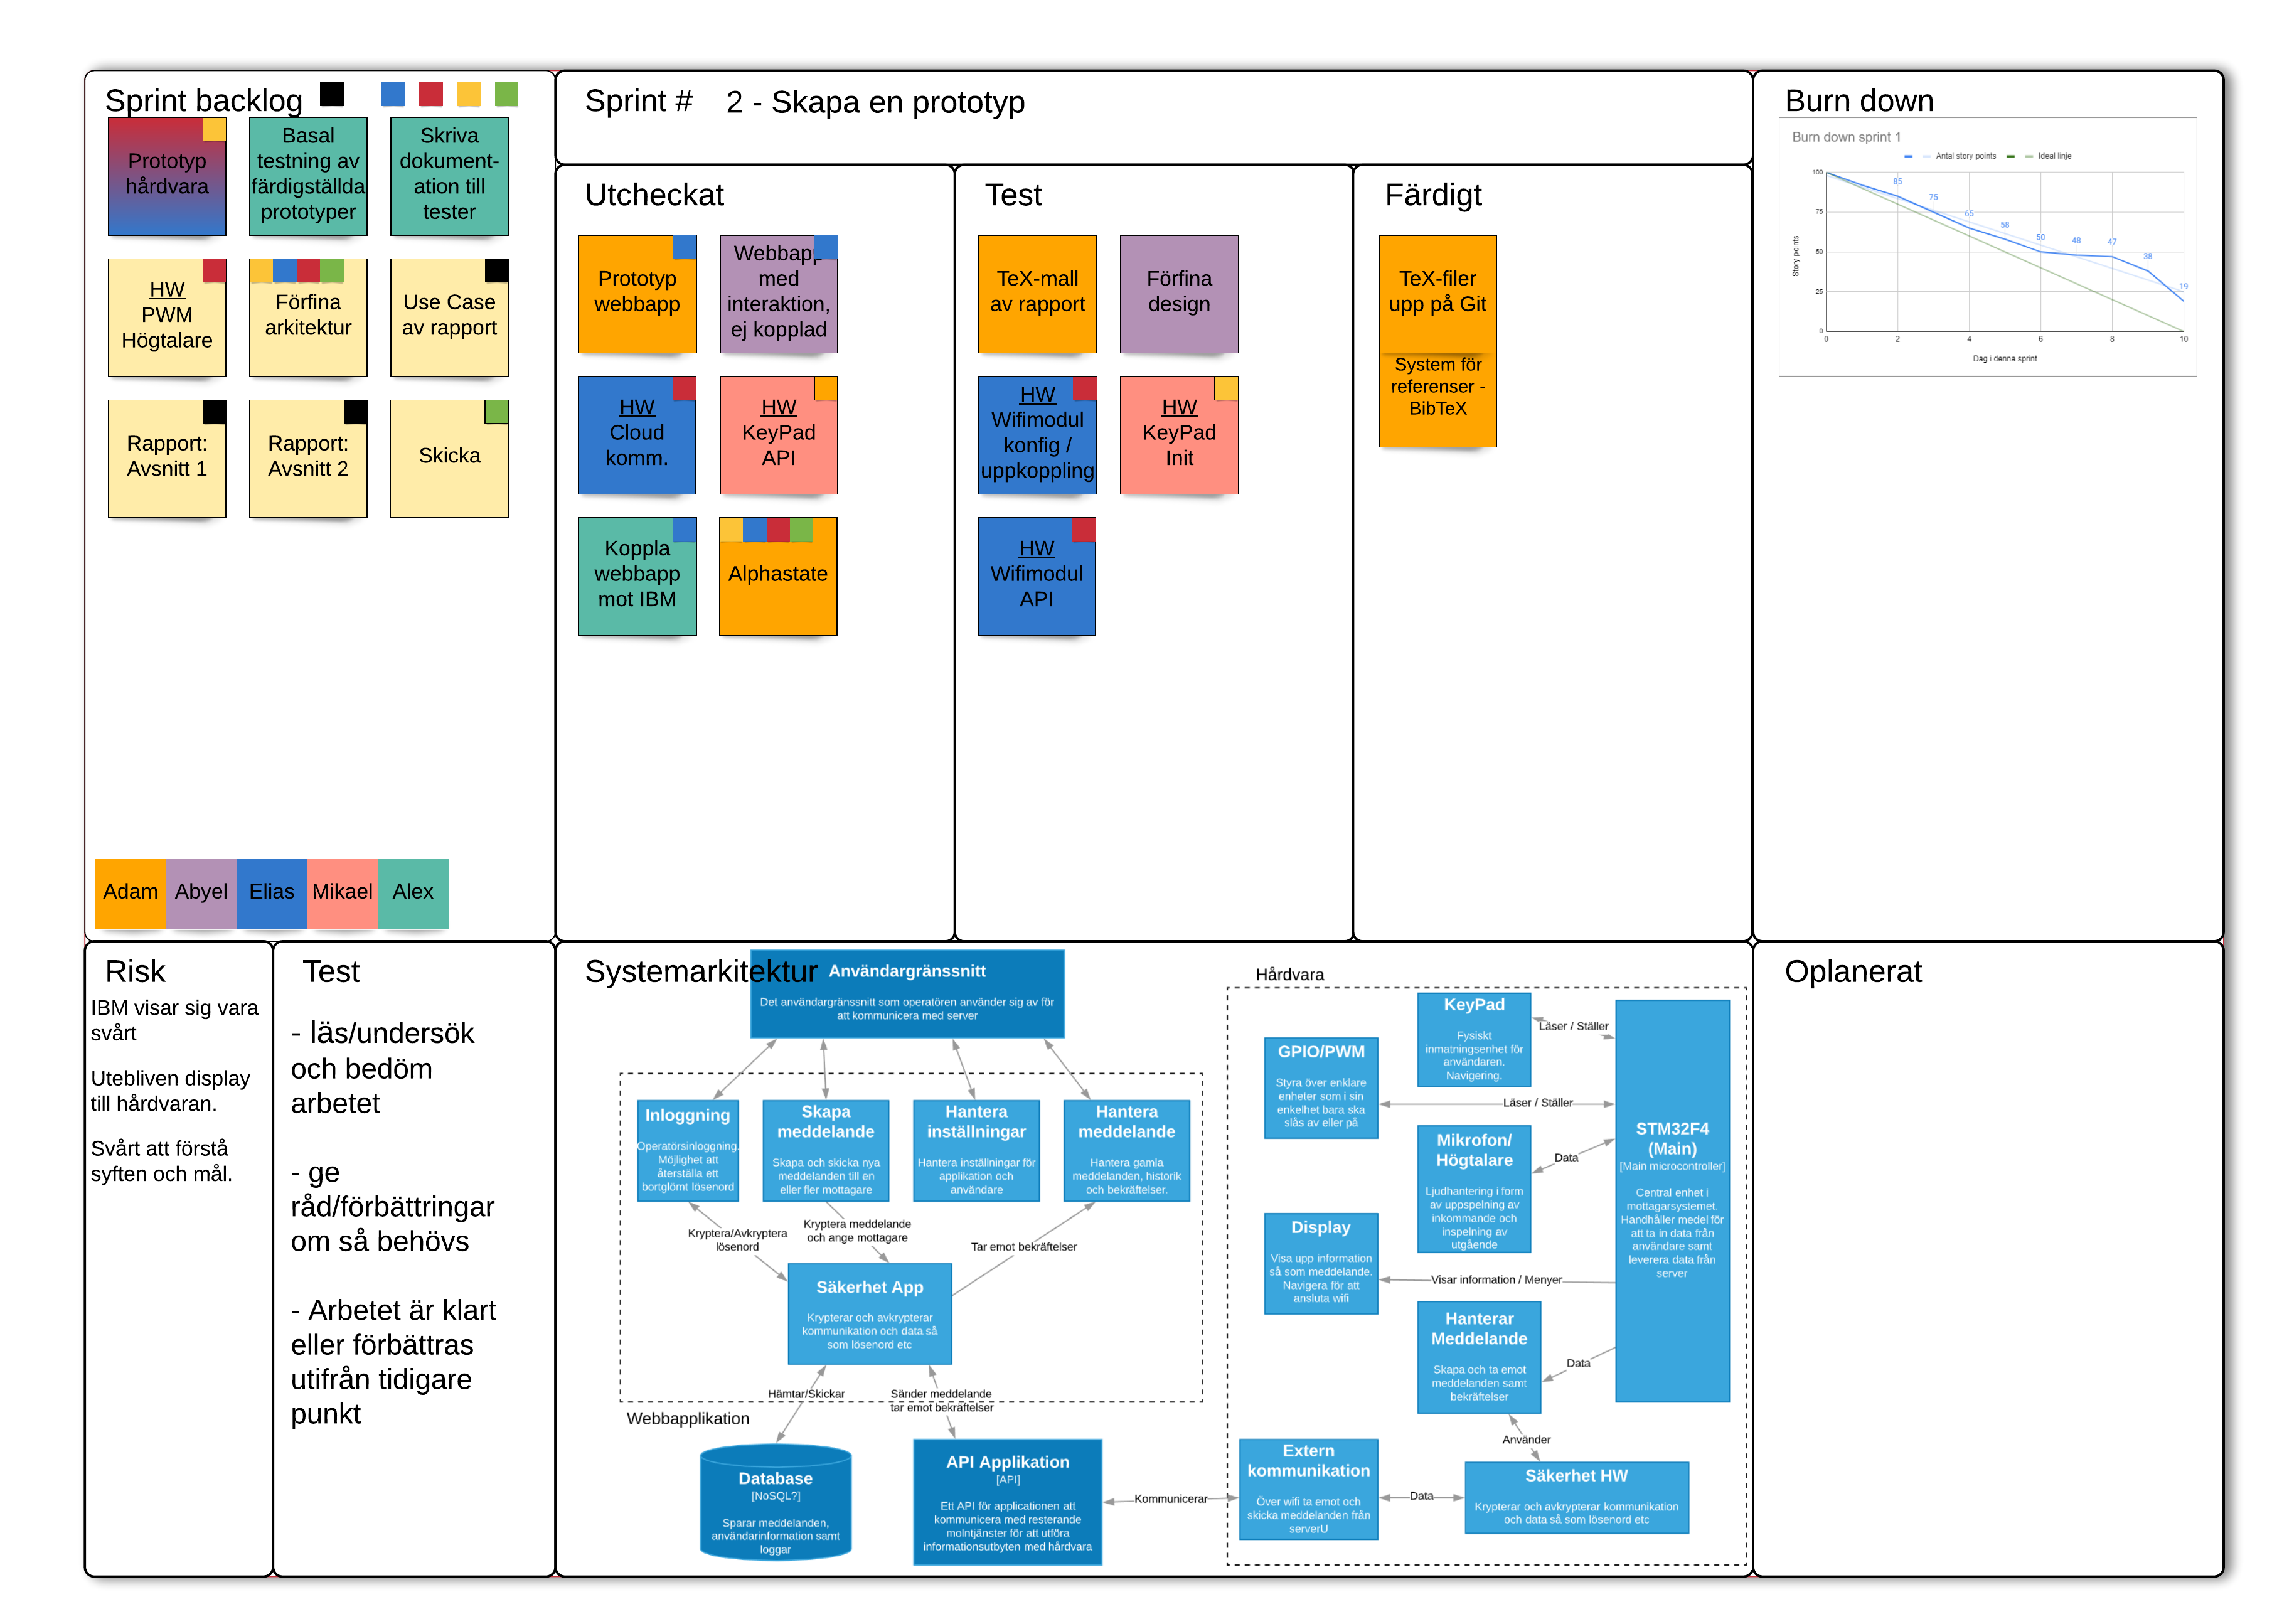
\includegraphics[max height=250px, max width=250px]{images/ArbetstavlaPrivat.png}}
    \caption{Arbetstavla, \textit{whiteboard}, \textit{Privat sida}}
    \label{fig:ArbetstavlaPrivat}
\end{figure}

\begin{figure}[htbp]
    \centerline{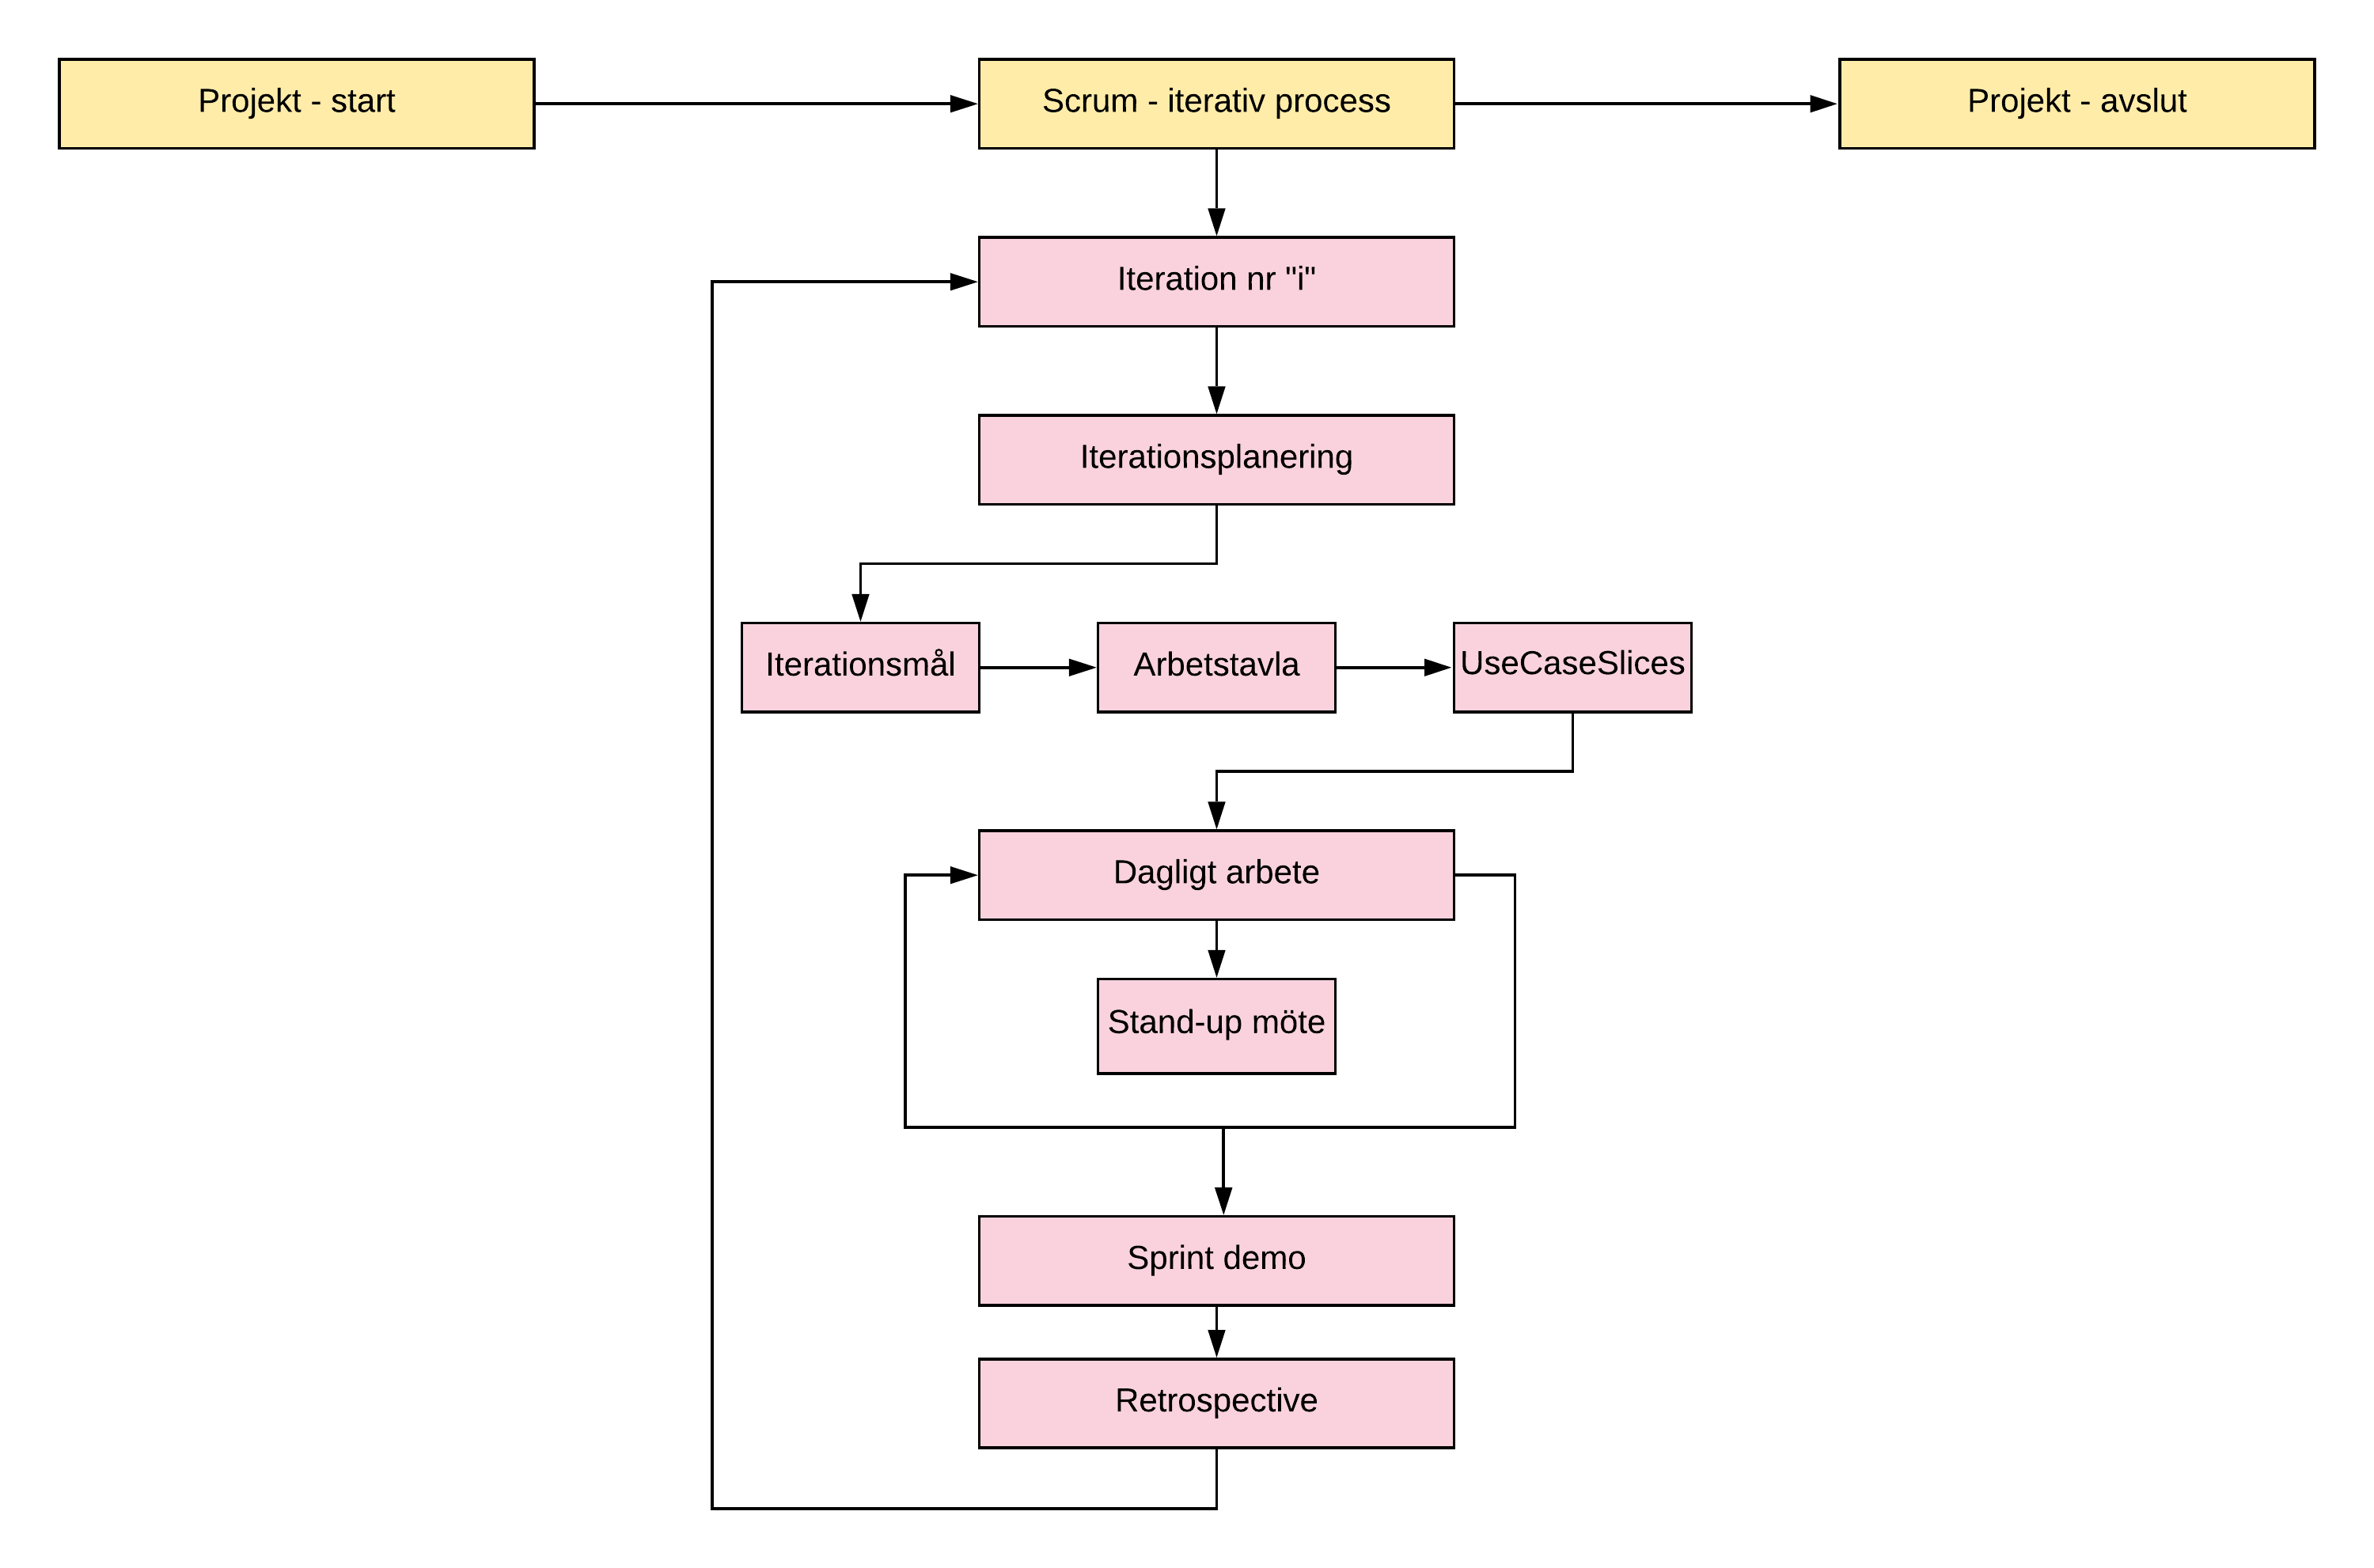
\includegraphics[max height=250px, max width=250px]{images/DiagramArbetsstruktur.png}}
    \caption{Projektgruppens egna övergripande arbetssätt i diagramformat.}
    \label{fig:DiagramArbetsstruktur}
\end{figure}

% Abyel
\section{Undersökningsmetoder}
Följande kapitel beskriver den metod som används i undersökningen för att hitta svar på problemformuleringen.
Metodens syfte är att hjälpa studenter hitta svar till ett antal följdfrågor, som har koppling till den större 
frågan om vad som utgör en bra projektmetod för små IT-projekt. Först anges de relevanta frågorna och sedan 
följer metodbeskrivning om undersökningsmetoden. 

% Abyel
\subsection{Frågor att besvara i undersökningen}
Följande frågor identifierades i slutet av varje iteration under projektarbetet, varav gruppmedlemmar diskuterade
om de metoder och praxis som passar bra för kommande iterationer samt de som ej bidragit till arbetet.
\begin{enumerate}
    \item Hur bedömer man om en projektmetod eller praxis är bra för små IT-projekt?
    \item Hur kategoriserar och namnger man 
    fungerande projektmetoder/praxis så att en gemensam diskussion kan föras med ingenjörer inom IT-området?
    \item Vilka ansvarsroller skall beaktas i undersökningen av projektet?
    \item Vilka moment och faser består ett projekt av och vilka metoder/praxis ska användas,
    undersökas och sedan bedömas?
\end{enumerate}

% Abyel
\subsection{Metodbeskrivning (undersökningsmetod)}\label{metodbeskr}
Då projektgruppen hade mindre erfarenhet inom projektarbete samt att varje projektgrupp tilldelats en förvald projektmetod utav kursen (se kapitel \ref{Bakgrund}), 
valde gruppen att genomföra undersökningen i form av en teoretisk studie, följd av praktiska tillämpningar av de metoder/praxis som identifierats 
i teoristudien. I studien analyserar gruppen tillgängligt kursmaterial i form av artiklar, kompendium, rapporter mm. Gruppen har även tagit del av 
material som presenterats inom föreläsningar, i form av projekt- och utvecklingsmetoder. Materialet har därefter diskuterats under s.k. \textit{sprint retrospectives}, 
möten som hålls inom slutet av varje iteration enligt SCRUM, där gruppmedlemmar jämfört modellerna och lyft upp deras för- och nackdelar.

Dessa metoder har, under godkännande av hela projektgruppen, använts i projektarbetet varav gruppen induktivt samlat in data om metodernas påverkan
och effekt till projektarbetet. På de retrospektiva SCRUM mötena för gruppen en diskussion om de metoder/praxis som använts, varav man beskriver metodernas 
fördelar samt nackdelar och påverkan till projektarbetet. I slutet av projektet sammanställdes allt resultat och ovannämnda diskussioner i en tabell 
(se tabell \ref{tab:bedomning}) där projektgruppen resonerar om de prövade metoder/praxis är passade för liknande små IT-projekt eller inte med motivering som grundar 
sig på erfarenhet från utförd projekt. Denna undersökningsmetod kan modelleras i ett UML-diagram, se figur \ref{fig:nyUndersökningsmetod}.

\begin{figure}[h!]
    \centerline{\includegraphics[max height=250px, max width=250px]{images/nyUndersökningsmetod.png}}
    \caption{Gruppens undersökningsmetod markeras som orange, inspiration från undersökningsmetod av kurs \textit{II1302 Projekt och projektmetod}}
    \label{fig:nyUndersökningsmetod}
\end{figure}

\textbf{Metod 1: Undersökningsmetod}.
Undersökningsmetoden består av ett antal formuleringar och steg som måste följas
för att uppfylla undersökningen och därmed hitta ett passande svar till problemformuleringen. Metoden består av följande 
sekvens som efterliknar en vetenskaplig arbetsmetod:
\begin{enumerate}
 	\item Ett problem inom ett ämnesområde identifieras och dess problemägare samt intressenter anges.
	\item Problemet formuleras och avgränsas, så att enbart faktorer och fenomen som rör problemet tas med.
    \item Relevant och befintlig kunskap samt existerande teori inom området samlas d.v.s information, metoder och 
    verktyg som kan stödja undersökningen.
	\item Problemformuleringen förklaras och en hypotetisk lösning presenteras med den samlade bakgrundskunskapen.
	\item Lösningsförslaget bearbetas med mer idéer och teorier varav en färdig lösning presenteras som kan testas i praktik.
	\item Testning av lösning och analys av dess resultat
    \item Lösningsförslag förbättras utifrån resultat. Om resultaten inte är tillräcklig eller otillfredsställande, 
    går man tillbaks till steg 4, samlar ny data och prövar nya hypoteser.
	\item Utvärdering av resultatet och jämförelse med existerande kunskap och data från liknande arbete, varav nya problemformuleringar
	kan identifieras for framtida undersökningar.
\end{enumerate}

Denna metod är anpassad för undersökningen som följer principer för vetenskaplighet i och med att den uppfyller följande krav:
\begin{enumerate}
    \item Objektiv: Metoden bör ge samma resultat förutsatt att den appliceras på projekt i liknande förutsättningar 
    (Projekt relaterat till IT, samma storlek på grupp mm).
    \item Kontrollerbar: Metoden kan kontrolleras utifrån alternativa metoder med villkor att de är anpassade för
    liknande situation.
    \item Teoretisk förankrad: Metoden är utformad utifrån gruppens teoristudie med kurslitteratur.
\end{enumerate}

Arbetsmetoden kan klassificeras inom \textit{tillämpad forskning}, då undersökningen är avgränsat inom området för ingenjörskonst och IT. 
Undersökningsmetoden har likt tillämpad forskning, syftet att ta fram ett konkret och användbart resultat som kan sättas 
i praktiken t.ex en produkt eller process/metod varav resultatet av denna undersökning ska motsvara en passande projektmetod för 
framtida små IT-projekt. Forskningen skiljer sig ifrån grundforskning, som är riktat mot generaliserat resultat som kan appliceras 
på flertal områden. Arbetsmetoden har i detta fall anpassats till att fungera jämsides med kursens projektarbete\cite{IT-BoF:3}\\

% Abyel
\textbf{Metod 2: Begrepp}.
För begreppsförråd så följer undersökningen mallen \textit{Essence language key} från Essential unified process (EssUP), 
en minimal, agil och iterativ mjukvaruutvecklings-process som innehåller nödvändiga praxis och metoder 
för att driva och genomföra projektarbete inom IT. Processen kan anpassas till små och stora projekt genom att 
lägga till eller ta bort praxis utifrån projektens krav \cite{Jacobson:4}. 
Se figur \ref{fig:ivar} och \ref{fig:essenceKey} som illustrerar dessa begrepp.

\begin{figure}[h!]
    \centerline{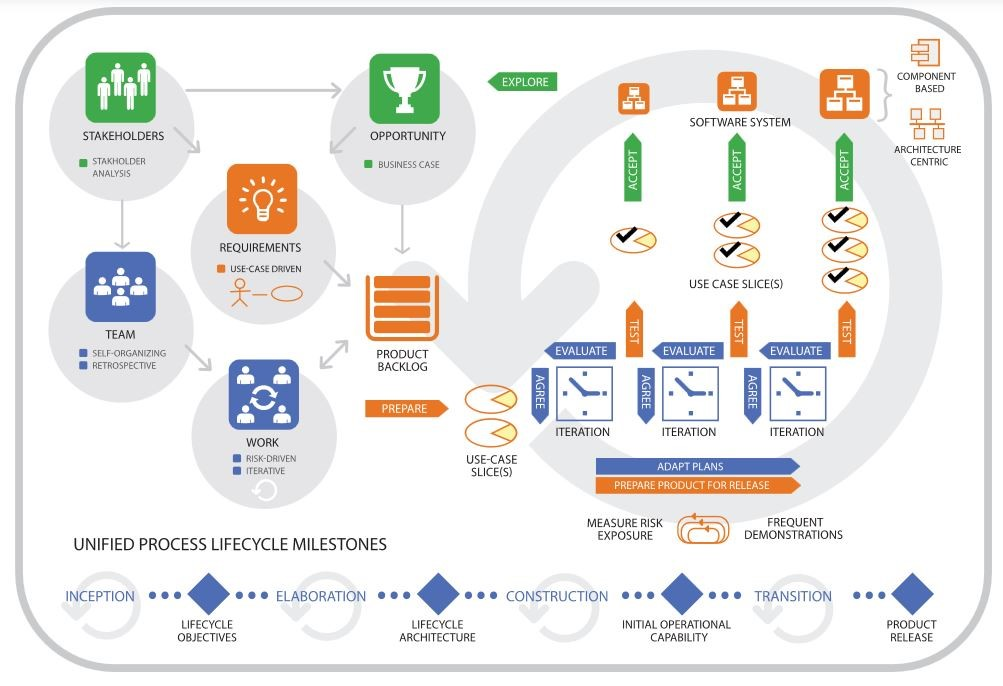
\includegraphics[max height=250px, max width=250px]{images/ivar.jpg}}
    \caption{Essential unified process}
    \label{fig:ivar}
\end{figure}

\begin{figure}[h!]
    \centerline{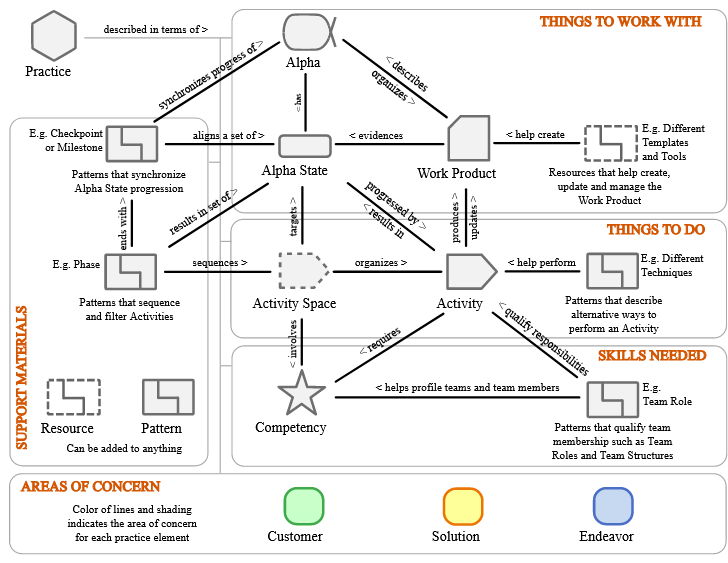
\includegraphics[max height=250px, max width=250px]{images/essenceKey.png}}
    \caption{Essential language key}
    \label{fig:essenceKey}
\end{figure}


% Mikael
\section{Genomförande}
Här redovisas viktiga beslut, förändringar och anpassningar i projektmetoden, praktikerna eller annat. För tydlighetens skull uppdelas detta kapitel i de ansvarsområden som fanns inom gruppen i detta projekt.

% Adam
\subsection{Projektledning (Adam)}
Gruppens projektmetod var som tidigare nämnts SCRUM, vilken var uppdelad i 5 iterationer om 2 veckor vardera. Dessa iterationer har till stor del följt den metod som beskrivs av Kniberg \cite{kniberg_scrum_2015}, där en iteration startar med en iterationsplanering följt av korta dagliga möten och avslutas med en reflektion över den iteration som gått.

Detta kan ses som ett flöde, där en iterationsplanering startar iterationen och gruppen därefter befinner sig inuti ett roterande flöde. Dagliga möten föregår arbetsuppgifter, som leder till nästa dags möte. När antingen tiden är slut eller arbetsuppgifterna är slut så kan iterationen sägas vara över, vilket leder till en iterationsreflektion som föregår nästa iterationsplanering. Därefter börjar nästa iteration enligt samma mönster. Se figur \ref{fig:iteration} för en flödesbeskrivning.

\begin{figure}[h!tbp]
    \centerline{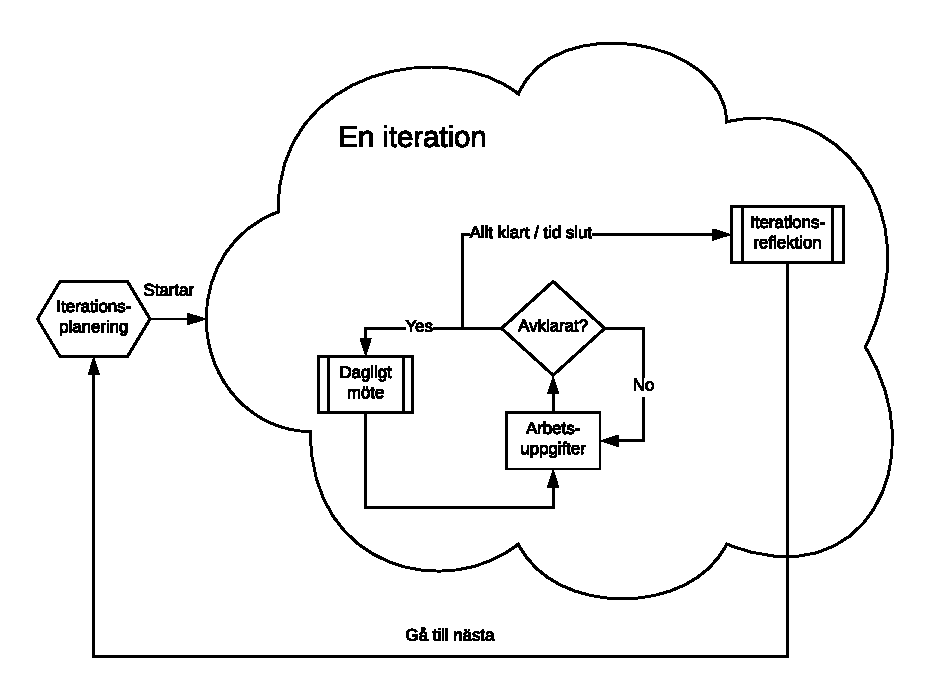
\includegraphics[max height=250px, max width=250px]{images/iteration.pdf}}
    \caption{Iteration/Sprint}
    \label{fig:iteration}
\end{figure}

De dagliga mötena syftade till att hålla koll på hur iterationen fortlöpt. Grunden i mötet var att varje deltagare skulle svara på följande:
\begin{itemize}
    \item Vad har du gjort sedan sist?
    \item Vad ska du göra nu?
    \item Behöver du hjälp?
    \item Behöver du uppdatera arbetstavlan?
\end{itemize}
Dessa möten hölls så korta som möjligt och syftade till att skapa bättre förutsättningar för att arbetsuppgifter skulle bli avklarade.

Iterationsreflektionsmötena utgick från arbetstavlan och de arbetsuppgifter som fanns där. Syftet var att finna vad som hade gått bra, vilka problem som uppstått och vad som skulle ändras till nästa iteration. Dessa möten var informella och hade inte någon direkt agenda, utan var mer ett diskussionsforum.

% Mikael
\subsection{Kund- och kravansvarig (Mikael)}
Efter att gruppen kommit överens om vilken produkt som skulle byggas så ställde kundansvarig upp en kravlista med skallkrav på produkten, samt en lista med önskemål på produkten. 
Utifrån denna lista skapades Stories och en användningsfallsmodell (UseCase model) och ur denna extraherades sedan användningsfall (UseCases) och till sist användningsfallsdelar 
(UseCaseSlices). Dessa UseCaseSlices mynnade ut i post-it-lappar på arbetstavlan som representerade arbetsuppgifter. Varje gruppmedlem fick en individuell bakgrundsfärg till 
post-it-lapparna och hörnen markerades med en färg som svarade mot det användningsfall som utgjorde grunden och skallkraven till produkten.
Under iteration tre så adderade gruppen några önskemål till kravlistan, vilket ökade komplexiteten något på produkten.     

% Elias
\subsection{Arkitekt (Elias)}
Under ett möte mellan webbapplikations- och hårdvarugrupperna togs de komponenter fram från vardera sida som behövdes för att skapa produkten. Dels de individuella gruppernas specifika delar men också de delar som behövdes för att dessa skulle i sin tur kunna kommunicera med varandra. En komponent här är en individuell praktiskt taget fristående del i systemet som kan utvecklas enskilt och sedan kopplas ihop med andra komponenter efter det att respektive är slutförd. Därefter användes dessa komponenter som byggblock i ett diagram där dessa grupperas in efter tillhörighet och riktningspilar placerade ut för att beskriva relationen mellan dessa. För att underlätta för både utomstående och utvecklare att förstå struktur och funktion så skapades ytterligare ett diagram där man flyttade upp en nivå i abstraktionslagerna. Genom att gruppera tillhörande komponenter till större block kunde en förenklad systembeskrivning därmed tas fram.

% Abyel
\subsection{Utvecklingsansvarig (Abyel)}
Utifrån systemarkitekturen, skapades detaljerade konceptuella modeller och strukturdiagram vars utformning är relevanta 
för de ramverk samt script- och programmeringsspråk som användes. Konceptuella modellen visar hur webbapplikationen ska utformas för webbutvecklare så att kravmål gällande applikationen uppfylls, medans strukturdiagrammet hjälper mjukvaruutvecklare skriva kod vars funktionalitet uppfyller målen i kravspecifikationen gällande produkten (pager). Då produkten 
består av två delprodukter som utvecklas i skilda miljöer så antogs beslutet att sätta upp två repositories i github varav de kan utvecklats 
utan risk för krock mellan källkoder. För utveckling så användes git för versionshantering och github för att sammanställa alla ändringar. 
När man jobbar med en \textit{checked out} task från arbetstavlan så skapar man separata brancher och jobbar med sin task tills den är klar, varav 
man gör en \textit{pull request} till orginal-branch (master). Under sådana fall testas och integreras det utförda arbetet med existerande arbete 
i master för \textit{live deployment}. 

% Alex
\subsection{Testansvarig (Alexander)}
Efter att webbapplikationen började komma på fötterna så valdes en lämplig teststrategi som lätt kunde adopteras av projektgruppen. Därefter skapades en testplan för att 
värdera vilka delar av webbapplikationen som bör testas, måste testas och som eventuellt kan testas om det finns tid och resurser. I början så valdes \textit{Jest} som 
testbibliotek för att skapa ett \textit{dummy test} för att se så implementationen fungerade som den var tänkt. Kort därefter togs beslutet att använda \textit{React Testing Library} 
då det skulle underlätta testandet av webbapplikationens DOM. Vid ett senare tillfälle under kursens gång så skedde det en förändring igen av testbibliotek, denna gång tillbaka 
till \textit{Jest}, detta skedde då projektgruppen kom fram till att tester av DOM inte kändes nödvändiga. Tester för de delar av system som krävde testning fungerade bra 
nog att enbart skrivas med hjälp av \textit{Jest}.

% Elias
\section{Resultat}
Målet var att hitta en bra projektmetod för små IT-projekt och det resultatet kan delas in i två delar. Det mest uppenbara är givetvis den resulterande metoden vi använde oss utav men även slutprodukten i sig själv är en del av det totala slutresultatet. Vid uppstarten hade vi 4 skallkrav och 16 önskemål att jobba emot. Inför slutdemonstrationen hade vi uppfyllt samtliga 4 skallkrav och över hälften, Dvs 9, av alla önskemål. Det i sig är en god indikator på att den metod vi använt har fungerat. För att göra en djupdykning i den projektmetod vi använt oss av finns det en lista på specifika delar som vi implementerat. Dessa kan ses i tabell \ref{tab:bedomning}. Här listas olika moment inom olika delar av projektmetoden, vad som har fungerat bra eller mindre bra samt vad alternativet skulle kunna tänkas vara.

\definecolor{green}{RGB}{0,204,0}
\definecolor{red}{RGB}{255,0,0}
\newcolumntype{L}[1]{>{\raggedright\arraybackslash}p{#1}}
\begin{table}[h!tbp]
	\caption{Bedömningstabell}
	\begin{center}
        \begin{tabular}{|L{0.15\columnwidth}|L{0.25\columnwidth}|L{0.25\columnwidth}|L{0.15\columnwidth}|}
            \hline
            \textbf{Ansvars-} & \textbf{Arbetssätt/metod} & \textbf{Omdöme} & \textbf{Alternativ} \\
            \textbf{område}& \textbf{praktik/mönster} & För- \& nackdelar & \\
            
            \hline
            
            Projekt- \break övergripande & 3st fasta arbetspass om 4 timmar i veckan & \textcolor{red}{Kan vara svårt att vara produktiv i sitt arbete när man har 4 studenter via Zoom} & Låt studenter planera sin egen tid \\
            
            \hline
            
            Analytiker & Arkitektur Överblick &\textcolor{green}{Ett väl abstraherat arkitekturdiagram ger god överblick av projektet i helhet} & Endast strukturera på lägre nivåer som delar av systemet \\
            
            \hline
            
            & Arkitektur komponentnivå & \textcolor{green}{Arkitekturen över individuella delar av systemet ger god möjlighet till tydlig arbetsindelning} & Använda enbart arbetstavla som systemindelning \\

            \hline

            & Arkitektur UML - Kodnivå & \textcolor{red}{I ett projekt som är av mindre storlek som detta blir det endast ett tidsödande moment som inte tillför värde} & Helt enkelt hoppa över detta steg helt då det inte används ändå \\
            
            \hline

            Utveckling & Särskilda repos för källkod i olika språk & \textcolor{green}{Håller delprodukt- \break er separerade utan risk för krock \& förlust av arbete} & Allt arbete \& wiki i ett repo (ej rekommenderat)\\
            
            \hline
            
            & Skapande av \textit{branch} med samma namn som utcheckad task samt Pull Request när task är slutförd & \textcolor{green}{Alla medlemmar jobbar utan risk att förstöra fungera- \break nde kod. Prototyp kan byggas inkre- \break mentellt.} & Jobba enbart i master-branch (ej rekommenderat) \\
            
            \hline
            
            & Konceptuell mo- \break dell och struktur- \break diagram till produkt & \textcolor{green}{Ge överblick över produktens kom- \break ponenter. Enklare att hitta tasks.} & \\
            
            \hline
            
            & &\textcolor{red}{Risk för lite an- \break vändning om modell är irrele- \break vant till produktens arkitektur.} & Dokumen-\break tation om hur komponenter skapas (ej rekommenderat) \\
            
            \hline
            
            & Dokumentering av tekniska komponenter & \textcolor{green}{Framtida underhåll och referens till projektarbeten} & Att inte dokumentera \\
            
            \hline
            
            Krav-\break ansvarig & Färgkodade UC och dess personer på arbetstavlan & \textcolor{green}{Skapar enkel överblick. En studie visar att enkla verktyg är populära. Samma studie visar att 26\% av tillfrågade IT-företag använde fysisk arbetstavla.\cite{SurveyofAgileTool}.} & Ett inte lika överskådligt sätt vore att inte skriva namn på UC och utvecklare. \\

            \hline

            Projekt-\breakövergripande mätbarhet av mål-\break uppfyllande & & \textcolor{green}{Produkten nådde alla 4 skallkrav samt 9 av 16 önskemål.} & Se bilaga K\\
            
            \hline
		\end{tabular}
		\label{tab:bedomning}
	\end{center}
\end{table}


% Adam
\section{Analys/Förbättringsförslag}\label{analys}
Gruppen har identifierat ett antal punkter där arbetet kunde ha fungerat smidigare, antingen genom andra arbetsmetoder
eller genom att ha bättre förkunskaper. Dessa punkter och förbättringsförslag listas här, och diskuteras vidare i
avsnitt \ref{diskussion}.

\subsection{Planering}\label{analys:plan}
Gruppen har saknat en långsiktig detaljerad planering för hela projektet, något som uppfattats som hämmande. Det har
funnits en planering för den produkt som skapats, men övriga uppgifter (såsom de formella dokumenten eller produktpresentationer)
har inte planerats mer än ytligt. Anledningen till detta är delvis att viss information inte har delgivits kursdeltagarna,
såsom vad som ska presenteras vid en kommande presentation, förrän bara några dagar innan iterationen startat. Med en
bättre framförhållning hade projektet som helhet kunnat planeras bättre, vilket sannolikt hade lett till högre effektivitet
och arbetsmoral.

\subsection{Versionshantering med Git}\label{analys:git}
När kursen startade var gruppmedlemmarnas kunskap om Git som versionshanteringsverktyg inte tillräcklig för det som har
krävts under projektets gång. Det läromoment om Git som ingår i kursen var heller inte tillräckligt eller relevant, 
utan fokuserade på andra delar av verktyget.

Gruppen saknade kunskap om hur man effektivt arbetar med \textit{pull requests}, \textit{branches} och \text{merge}.
Tidigare arbete med Git har varit mindre komplext och läromomentet berörde dessa delar för ytligt eller inte alls,
varför kunskaperna inte räckte till.

Detta var särskilt tydligt vid arbetet med denna rapport, som gruppen valde att skriva i \LaTeX\:med hjälp av Git. Problemet uppstod då arbetet sker i samma fil vilket lättare skapar konflikter.

För kommande kursomgångar föreslår gruppen att läromomentet revideras och istället fokuserar mer på hur man som grupp arbetar med Git och vilka hjälpmedel det finns, till exempel \textit{mergetool} och tillägg till mjukvara, såsom \textit{GitLens} till \textit{Visual Studio Code}.

\subsection{Serverplattform}\label{analys:server}
Gruppen använde initialt \textit{IBM Cloud} som serverplattform, och lade värdefull tid på att lansera produkten med hjälp av plattformen. Av olika skäl lyckades dock inte gruppen med detta, utan valde att använda \textit{Firebase} som serverplattform och \textit{GitHub Actions} för \textit{CI/CD}.

Att valet föll på \textit{Firebase} var för att delar av gruppen använt det i en tidigare kurs, och upplevt att det var en enklare plattform att jobba med än \textit{IBM Cloud}. Gruppen vill understryka att de inte är emot att lära sig nya plattformar, men känner att det var otydligt att valet av serverplattform var upp till gruppen. Hade detta varit tydligt hade gruppen sannolikt valt den nuvarande lösningen direkt, och därmed sparat tid som kunde lagts på att förbättra produkten.

\subsection{Modellering}\label{analys:modell}
Gruppen skapade initialt ett antal modeller över produkten och dess beståndsdelar, men i takt med att produkten utvecklades uppdaterades inte modellerna till att representera verkligheten. I efterhand önskar gruppen att den hade använt modellerna mer och jobbat fram en tydligare arkitektur. Med hjälp av denna skulle gruppen sedan ha skapat produkten utifrån arkitekturen, istället för att som nu behöva justera arkitekturen efter produkten. En tänkbar anledning till detta är att modellernas vikt inte tagits upp vid presentationerna, varför de prioriterats bort.

\subsection{Mäta utveckling}\label{analys:chart}
För att mäta utvecklingen under projektets gång användes \textit{burn down chart}, där tanken var att varje arbetsuppgift på arbetstavlan hade samma vikt. I takt med att arbetsuppgifter avklarades skulle därmed en tydlig trend kunna visas i grafen, där en något sånär linjär linje går mot noll från startvärdet (som representerar den iterationens antal uppgifter).

Gruppen uppfattade emellertid att denna mätning inte tillförde särskilt mycket. Det var enkelt att se utvecklingen genom att dels titta på arbetstavlan och se hur antalet avklarade uppgifter ökade, dels genom att se hur produkten utvecklades. Utöver detta var mätningen svår att underhålla, då nya uppgifter fick läggas till allt eftersom iterationen pågick.

% N/A
\section{Diskussion}\label{diskussion}
Detta kapitel diskuterar metod, resultat och bidrag till vetenskaplighet.

% Here you can define your own colors to use in the table. 
\definecolor{grey}{RGB}{217,217,217}

\begin{table}[h!tbp]
	\caption{Keep - Problems - Try\break\textit{Roll - student}}
	\begin{center}
		\begin{tabular}{|L{0.15\columnwidth}|L{0.25\columnwidth}|L{0.25\columnwidth}|L{0.15\columnwidth}|}
			\hline
			\multicolumn{4}{|c|}{\cellcolor{grey}\textbf{Keep}}\\
			\hline \rowcolor{grey}
			\textbf{Keep}                         & \textbf{Motivation}      & \textbf{Förbättringar} & \textbf{Referenser} \\
			\hline
			En fysisk (om än i molnet) arbetstavla &För överblickens skull.&Enklare färgsättningssystem. T.ex. färgmarkera ramen runt \text{tasks} istället för ena hörnet.&[Källa: Survey of Agile Tool Usage and Needs]\\
			\hline
			Separata repositories för källkod i olika programmeringsspråk&
            Enklare att separera delprodukter, Större sammanhållning bland delar&& \\
			\hline
			Skapande av branch med samma namn som utcheckad task&
            Separerar kod i utveckling från fungerande kod, eliminera risk att förstöra fungerande prototyp&                     & \\
			&                          &                     & \\
			\hline
			
			% This is a separator, since the tables in the .doc-template are labeled as the same table.
			\multicolumn{4}{c}{}\\
			
			\hline
			\multicolumn{4}{|c|}{\cellcolor{grey}\textbf{Problems - Try}}\\
			\hline \rowcolor{grey}
			\textbf{Problem}                      & \textbf{Try what?}      & \textbf{Motivering} & \textbf{Referenser} \\
			\hline
			Versions-hantering med GitHub. Versions-konflikter&
			Skapa plan innan rapportskrivning för hantering av versionskonflikter&
			För att minimera felaktigheter och tidsförlust vid rapportskrivandet& \\
			\hline
			Svårt att avgöra hur lyckad en praxis/metod är. Burn-down-chart fungerade inte fullt ut&
			Bestäm en annan typ av mätskala på hur väl projektet fungerar innan uppstart&
			För att få feedback på vilken effekt ändringarna har& \\
			\hline						
			
			% This is a separator, since the tables in the .doc-template are labeled as the same table.
			\multicolumn{4}{c}{}\\
			
			\hline
			\multicolumn{4}{|c|}{\cellcolor{grey}\textbf{Problems - Skip}}\\
			\hline \rowcolor{grey}
			\textbf{Problem}                      & \textbf{Skip or}        & \textbf{Motivering} & \textbf{Referenser} \\
			\rowcolor{grey}                         & \textbf{replace, why?}  &                     &  \\
			\hline
			Skapa arkitektur UML diagram ner på kodnivå&
			Tidsödande utan att tillföra mervärde för projektet&
			Det övergripande arkitekturdiagrammet ger bra överblick, men på kodnivå användes den inte& \\
			\hline
			Flera långa styrda arbetspass varje vecka&
			Ibland svårt att få arbetsro för vissa uppgifter om hela gruppen sitter ihop&
			Drivna studenter kommer att dra sitt strå till stacken utan att övervaka varandra. Tilliten ökar och därmed effektiviseras arbetet&
			Avsnitt 7.9.3 \cite{Eklund:2} \\
			\hline
		
		\end{tabular}
		\label{tab1}
	\end{center}
\end{table}

% Abyel
\subsection{Metoddiskussion}
Undersökningsmetoden innebär kort att gruppen gör en teoretisk studie av existerande metoder/praxis, varav man diskuterar deras för- och nackdelar samt applicerar de på projektarbetet där man analyserar deras inverkan på arbetet. Genom att utföra metoden på sekvensen i kapitel \ref{metodbeskr}, som efterliknar en vetenskaplig arbetsmetod, samt följa principer för vetenskaplighet: objektiv, kontrollerbar och teoretisk förankrad så stärks metodens \textit{validitet}. Detta via den samlade teoretiska kunskapen och gemensamma erfarenheten.

Däremot kan metodens \textit{reliabilitet} ifrågasättas då gruppen enbart fick applicera metoder/praxis till en förutbestämd projektmetod med en satt iterationslängd. I och med dessa krav så rörde sig projektet mot ett riktat håll och därmed mot ett förutbestämt resultat, därav blev det svårt att hitta ett tillförlitligt svar till problemformuleringen för alla IT-projekt. Saker som gruppdynamik, attityd och tillgänglighet kan också spela roll för reliabiliteten, varav sådana faktorer påverkar hur medlemmar utvärderar den prövade metoden och praxis. Den rådande coronaepidemin är också en faktor då undersökningen (samt projektarbetet) skedde på distans utan fysiska träffar under hela projektet. I och med att liknande undersökningar utförs av flera studenter bör metodens relativitet vara säker. 

Sammanfattningsvis hjälper denna undersökningsmetod projektgrupper, med liknande problemformulering, att studera metoder/praxis och praktiskt tillämpa de i ett projektarbete varav metoderna kan utvärderas efter varje iteration. Metoden bör ge validitet och reliabilitet, förutsatt att undersökningen tillåts experimentera med flera projektmetoder och intervallet på iterationer. Tabell \ref{tab1}, baserad på gruppens resultat i tabell \ref{tab:bedomning}, bidrar med metoder och praxis som rekommenderas att prövas, problemfall som kan lösas genom alternativa metoder eller i vissa fall ta bort metoder.

% Elias
\subsection{Resultatdiskussion}
Att göra en bedömning av resultatet för utfört projekt visar sig inte vara helt enkelt och inte heller fullt ut rättvis. Till att börja med var uppgiften att utvärdera och testa sig fram till den projektmodell som fungerar bäst för små IT-projekt men vi var från början styrda mot en relativt specifik och fördefinierad modell. Detta orsakar både omedvetet och till viss del medvetet ett riktat testförfarande med en given utgångspunkt. Huruvida detta upplägg kanske är ett måste för att begränsa projektet och testningen av projektmodeller utifrån den tidsram som finns är öppet för diskussion. Den diskussionen ligger dock utanför denna rapport men den utgångspunkten är en viktig del att ha med sig mycket på grund av att det är svårt att hitta ett resultat som är mätbart och kommer därför bestå till stor del av åsikter snarare än vetenskapliga mätningar.

Ett sätt att faktiskt försöka få ut ett direkt mätbart resultat för att så sätt delvis bedöma detta är att jämföra de initiala kundkrav som ställdes i specifikationen mot den produkt som stod färdig vid den slutliga sprintdemonstationen. Se bilaga K (Kravspecifikation) för fullständig kravlista. I denna fanns det fyra skallkrav vars uppfyllande var ett minimikrav för att produkten skulle kunna anses som färdig produkt i någon form alls. Utöver dessa fanns det ytterligare 16 önskvärda krav som innehåller extra funktioner som kunden önskade få implementerade utefter bästa mån av tid och kostnad. I detta projekt hade vi dock en begränsad mängd tid att utnyttja och man kan därför anse att kostnadsaspekten också var ett mått av tid. Gruppens resultat i relation till kravspecifikationen blev i slutändan
\begin{itemize}
	\item 4 av 4 skallkrav uppfyllda
	\item 9 av 16 önskvärda krav uppfyllda
\end{itemize}
Att mäta slutprodukten på detta sättet kan säga oss ganska mycket i generella termer om projektmetoden utan att gräva ner sig och göra djupgående analyser i detaljerna. Samtliga skallkrav är uppfyllda och över 50\% av extra önskvärda tillägg visar att arbetet har fungerat bra och lett till goda resultat i slutprodukten. 

Givetvis behöver vi även analysera andra aspekter av projektmetoden än den slutgiltiga produkten för att förstå vad som har fungerat bra och mindre bra. I tabell \ref{tab:bedomning} listas olika delar av metoder i arbetet tillsammans med både för- och nackdelar samt eventuella förändringar som kan tänkas göras i dessa eller helt enkelt alternativa lösningar. Det vi tydligt kan se är att den grundläggande modellen med ett flertal mindre modifieringar utgör tillsammans en enkel men effektiv projektmodell att jobba utifrån. Nyckeln till en lyckad modell när man jobbar i små grupper med små projekt är att hitta modellen lagom. Man vill använda de hjälpmedel som tillför mer värde till arbetet än vad de kostar att utföra. Arkitekturdiagrammen är ett bra exempel på detta där de mer abstraherade diagrammen ger en god överblick med möjlighet till tydlig arbetsindelning medans de specifika och detaljerade diagrammen kostar mycket att skapa och tillför nästan ingenting.

Under arbetets gång hittades flera små förbättringar som gjorde arbetet lättare. Färgkodning var till exempel ett moment som infördes på flera ställen för att ge tydlig uppdelning redan på överblicksnivån. Både Use Case och Stories utnyttjade denna förbättring på arbetstavlan och resulterade i att man snabbt och enkelt kunde se vad som pågick och vem som gjorde det. En viktig aspekt som man inte får glömma är att när vi pratar om grupper och projekt såhär små så är modellen i högsta grad beroende av projekttyp och utvecklarna som deltar. I väldigt stora projekt inom mellanstora till stora team så är en förutbestämd struktur och metod ett absolut krav. Men i detta fallet måste det finnas något spelrum att arbeta inom för att uppnå bästa effektivitet. Det vill säga att det kan vara svårt att sätta fingret på en specifik metod med särskilda förhandsdefinierade detaljer som ska passa alla typer av projekt och människor. Med det sagt så har vi definitivt hittat en metod som passade gruppen för det projekt vi jobbade på och den miljö vi jobbade i just då.

% Alex
\subsection{Bidrag till vetenskaplighet, ingenjörserfarenhet, studenterfarenhet}
Projektgrupp 8 anser att skapandet av denna rapport bidragit med vetenskaplighet då denna undersökning av \textit{Vad är en bra projektmetod för små IT-projekt?} har undersökts 
på ett systematiskt och metodiskt sätt inhämtat kunskap om projekt och projektmetoder genom givet kursmaterial och kurslitteratur. Detta arbete har bidragit med ingenjörserfarenhet 
till varje projektmedlem genom undersökning och påläsning om projekt och projektmetoder som används idag i arbetslivet på ett brett spektrum av företag, utförandet av IT-projektet 
har även bidragit till ingenjörserfarenhet. Gällande studenterfarenhet så har detta arbete utvecklat projektmedlemmar genom mer erfarenhet inom olika verktyg som ex. 
versionshanteringsverktyg, \LaTeX\:och mm.

% Abyel
\section*{Slutord}
Projektgruppen avslutar denna rapport med att reflektera över det projektarbete och undersökning som genomförts. Via kursen \textit{II1302 Projekt och Projektmetoder} har gruppen förfinat sina tidigare kunskaper om projektarbete från kurs \textit{II1300 Ingenjörsmetodik} samt lärt sig om existerande projektmetoder. Gruppen har fått chans att föreslå användbara och beprövade praxis samt anpassa en projektmetod utifrån projektets storlek, längd, område mm. Var och en har även lärt sig betydelsen av ansvarsroller och hur man deltar, leder och organiserar ett projektarbete utifrån ens roll. Gruppen har dessutom visat en stor sammarbetsförmåga i och med att gruppdynamiken
fungerat bra utan några konflikter. Därav är gruppen på god väg att uppfylla kursens examinationsmål och ett steg närmare att bli utbildade ingenjörer, redo att delta i eller organisera egna projektarbeten ute i arbetslivet.

Via de analyser och resultat som genererats av den utföra undersökningen har guppen även bidragit till vetenskap och ökat kunskaperna inom ingenjörskonst och projektmetodik, en kunskap som man hoppas framtida studenter kommer ta del av under deras egna projektarbeten.\\

\vspace{12pt}

% You can switch citation style. ieeetran could be useful, as it is a bit more pleasing to the eyes.
\bibliographystyle{apalike}
\bibliography{references}

\newpage

\appendix
\textbf{Formella dokument}\\
A: Adam Liliemark, projektledare\\
B: Elias Johansson, arkitekt\\
C: Mikael Andersson, kravansvarig\\
D: Abyel Tesfay, utvecklingsansvarig\\
F: Alexander Jonsson, testansvarig

\textbf{Tekniska dokument}\\
F: Adam Liliemark, cloud functions\\
G: Elias Johansson, wifi\\
H: Mikael Andersson, knappsats\\
I: Abyel Tesfay, redux actions\\
J: Alexander Johansson, tester

\textbf{Övriga bilagor}\\
K: Kravspecifikation\\
L: Projektdefinition

\newpage

\onecolumn

\begin{appendix}
    \begin{center}
        \large
        A:\\Formellt dokument: Adam Liliemark, projektledare
    \end{center}

    \clearpage
    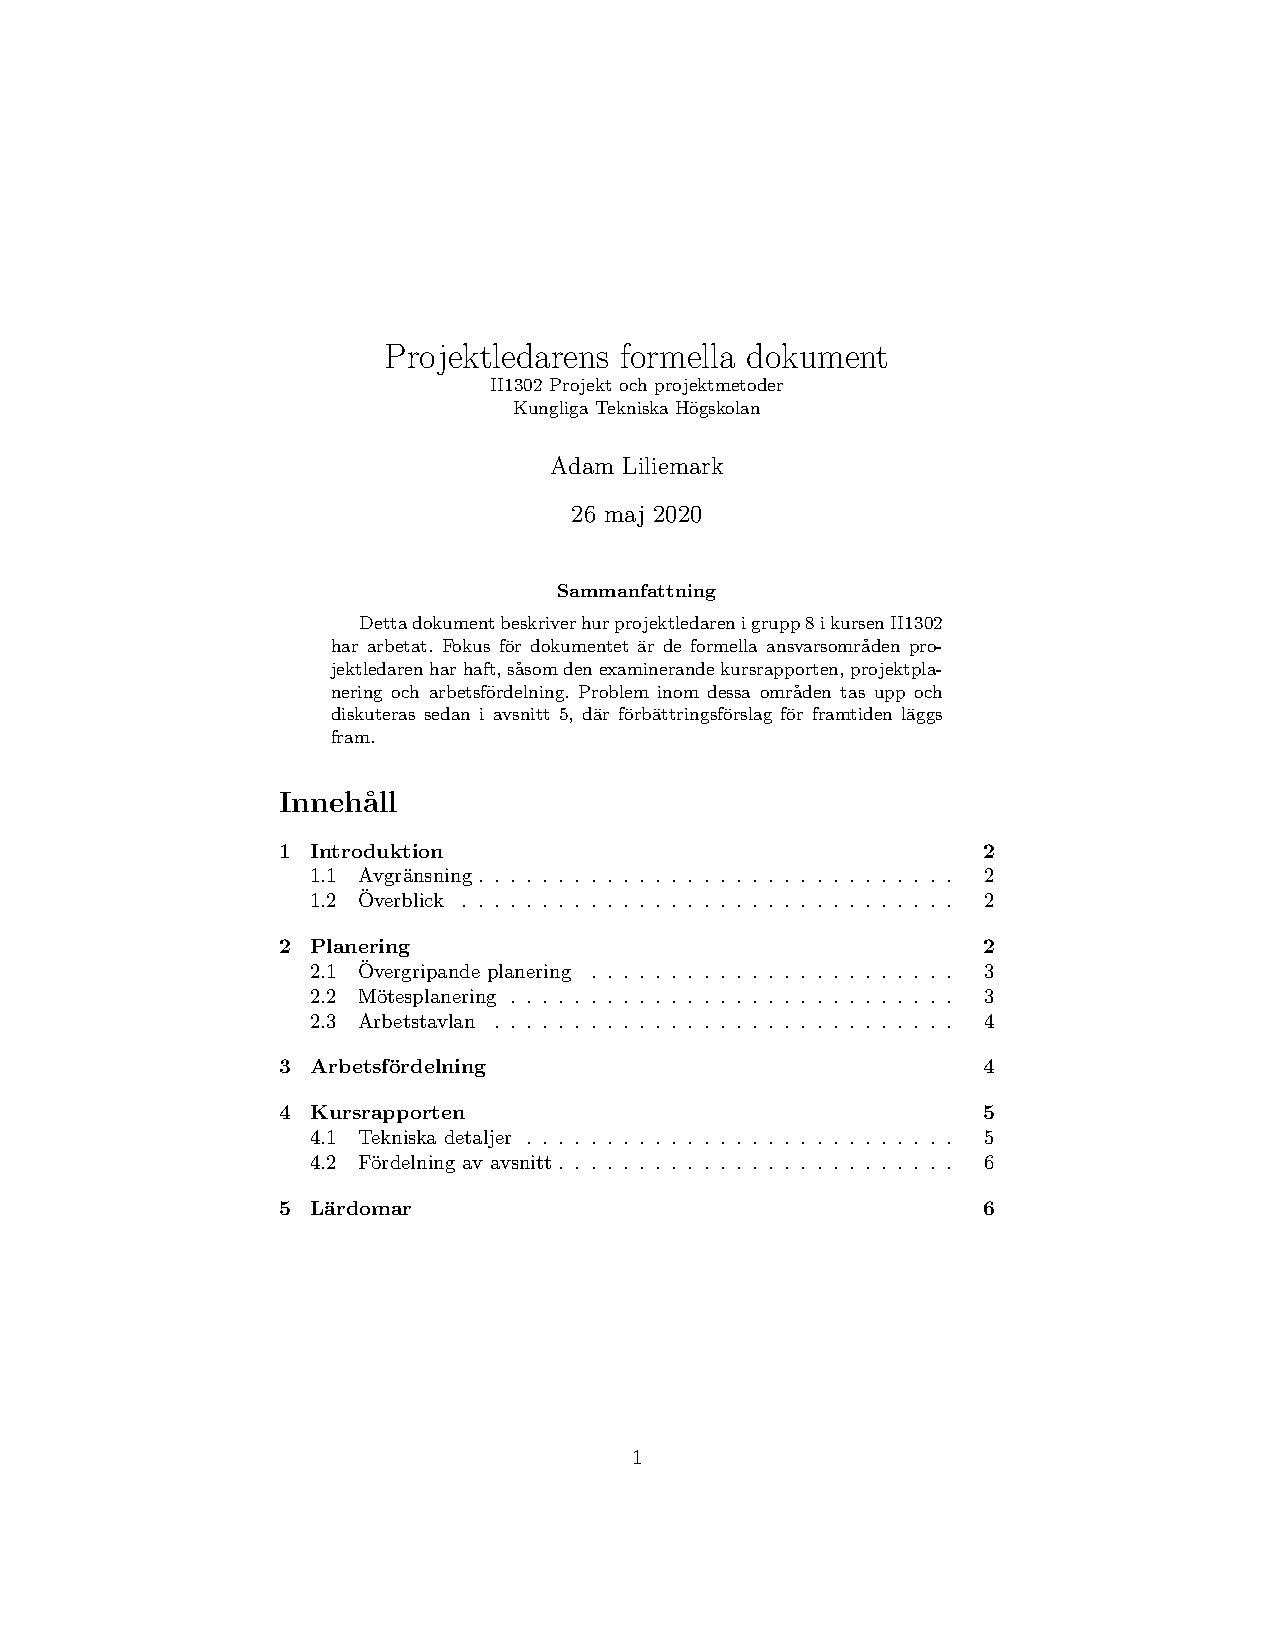
\includepdf[pages=-]{appendix/formell_al.pdf}
\end{appendix}

\begin{appendix}
    \begin{center}
        \large
        B:\\Formellt dokument: Elias Johansson, arkitekt
    \end{center}

    \clearpage
    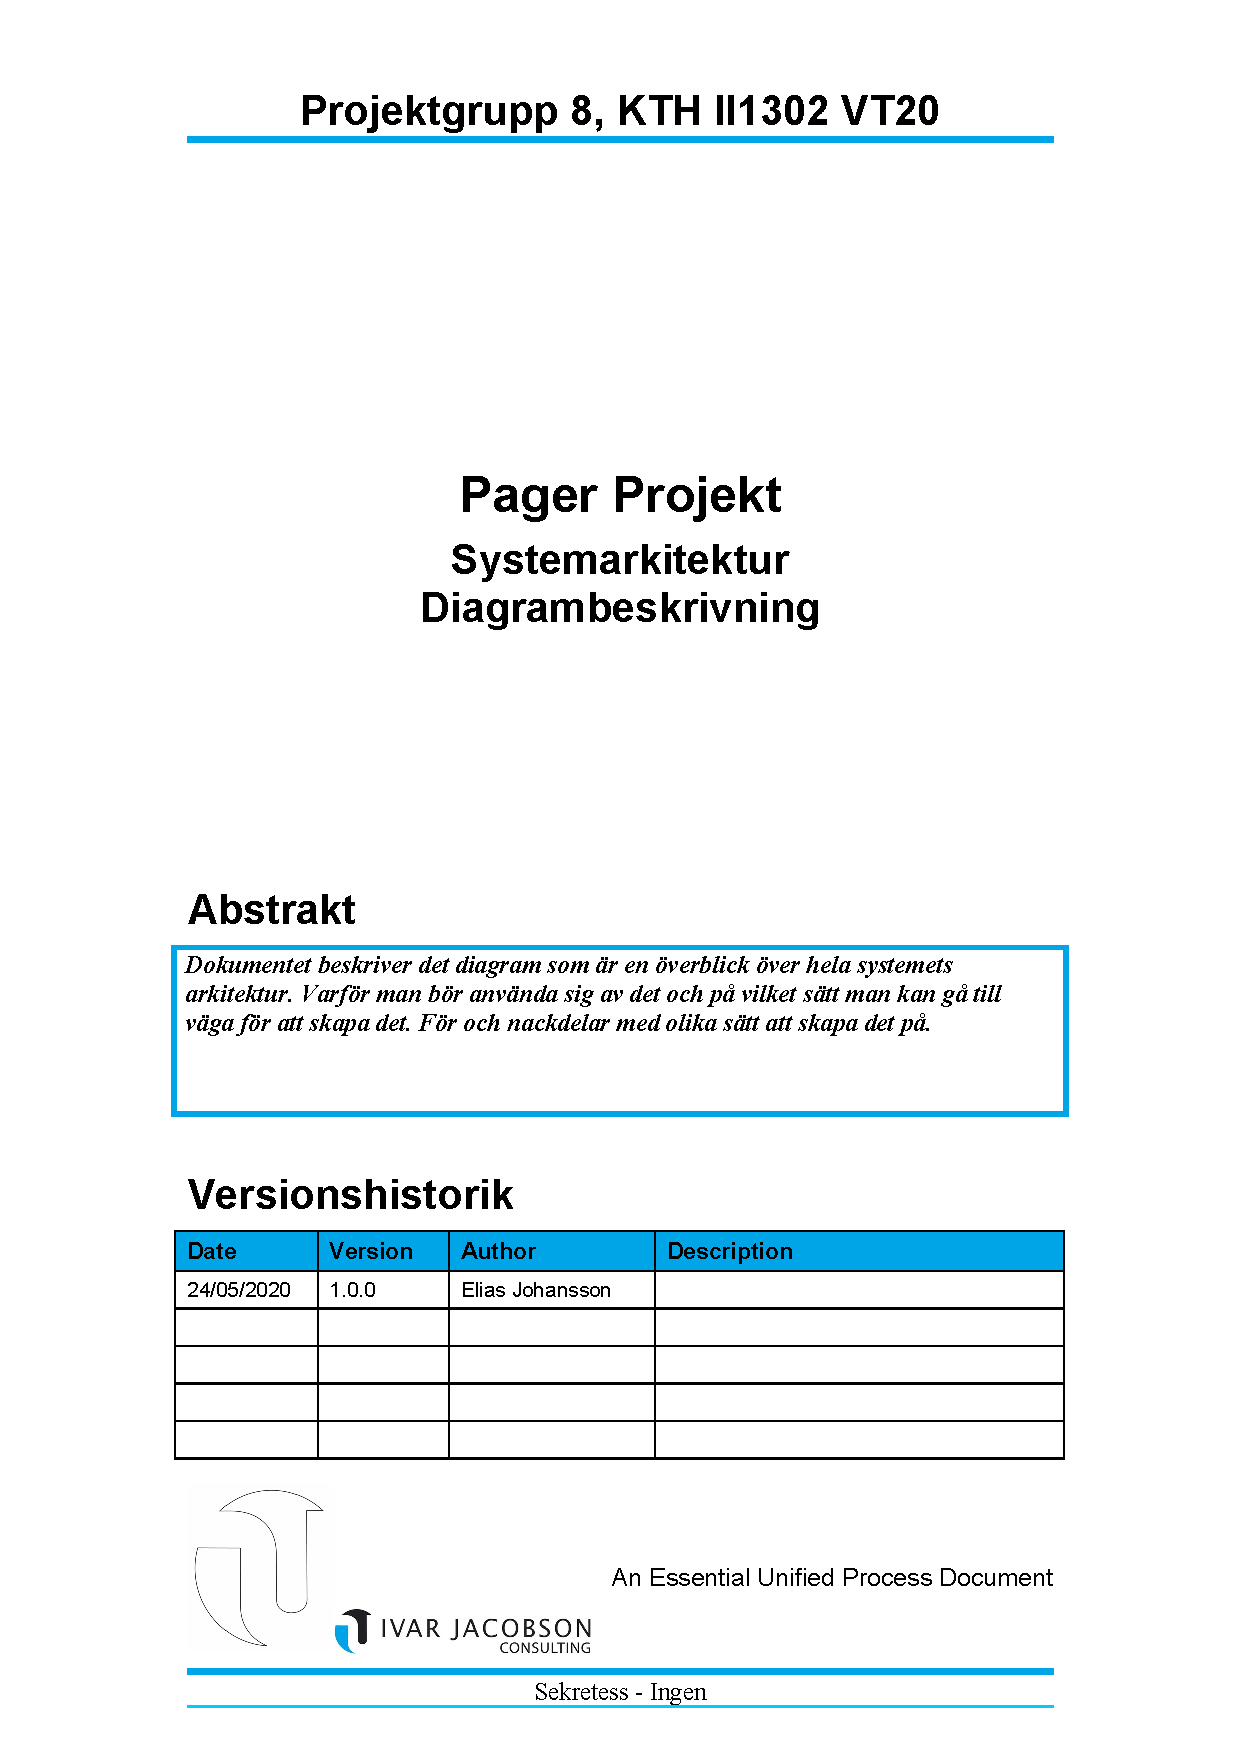
\includepdf[pages=-]{appendix/formell_ej.pdf}
\end{appendix}

\begin{appendix}
    \begin{center}
        \large
        C:\\Formellt dokument: Mikael Andersson, kravansvarig
    \end{center}
    
    \clearpage
    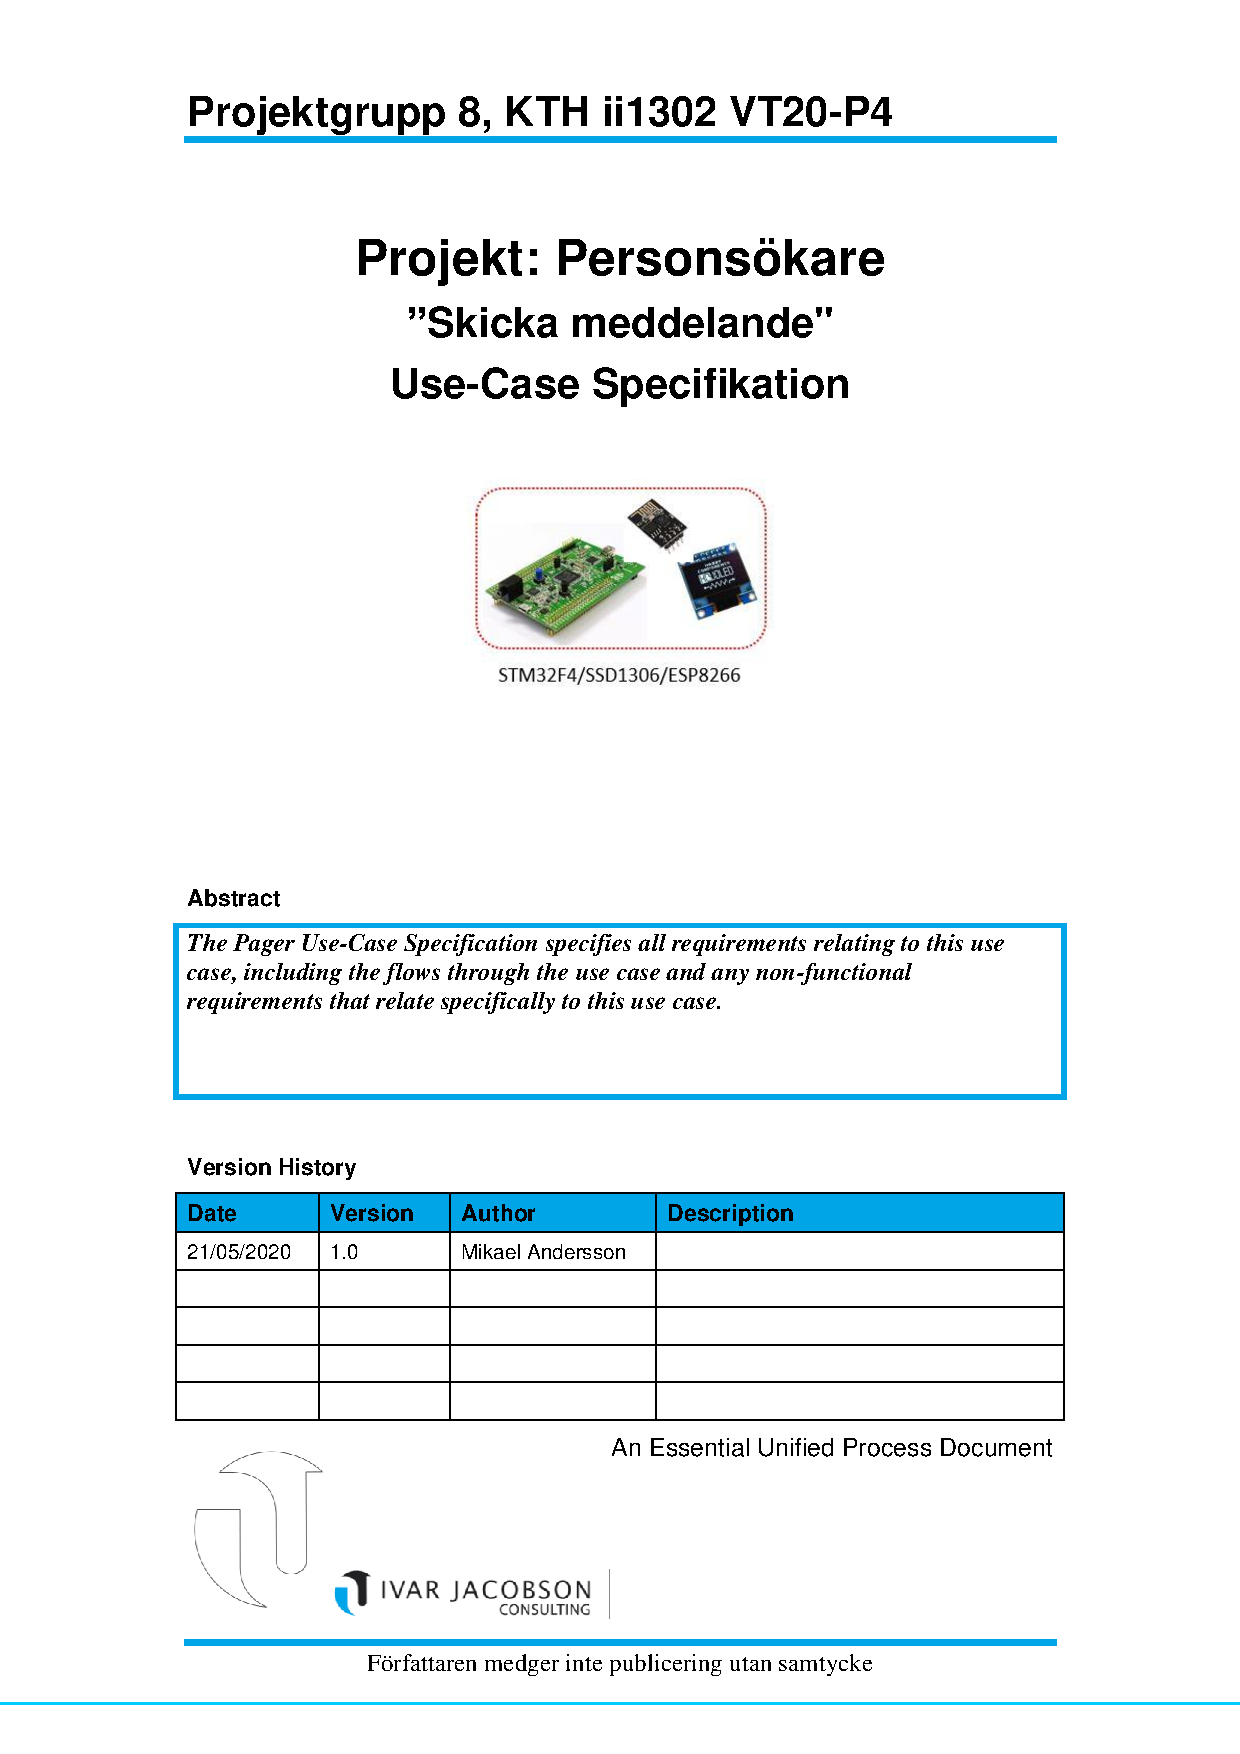
\includepdf[pages=-]{appendix/formell_ma.pdf}
\end{appendix}

\begin{appendix}
    \begin{center}
        \large
        D:\\Formellt dokument: Abyel Tesfay, utvecklingsansvarig
    \end{center}

    \clearpage
    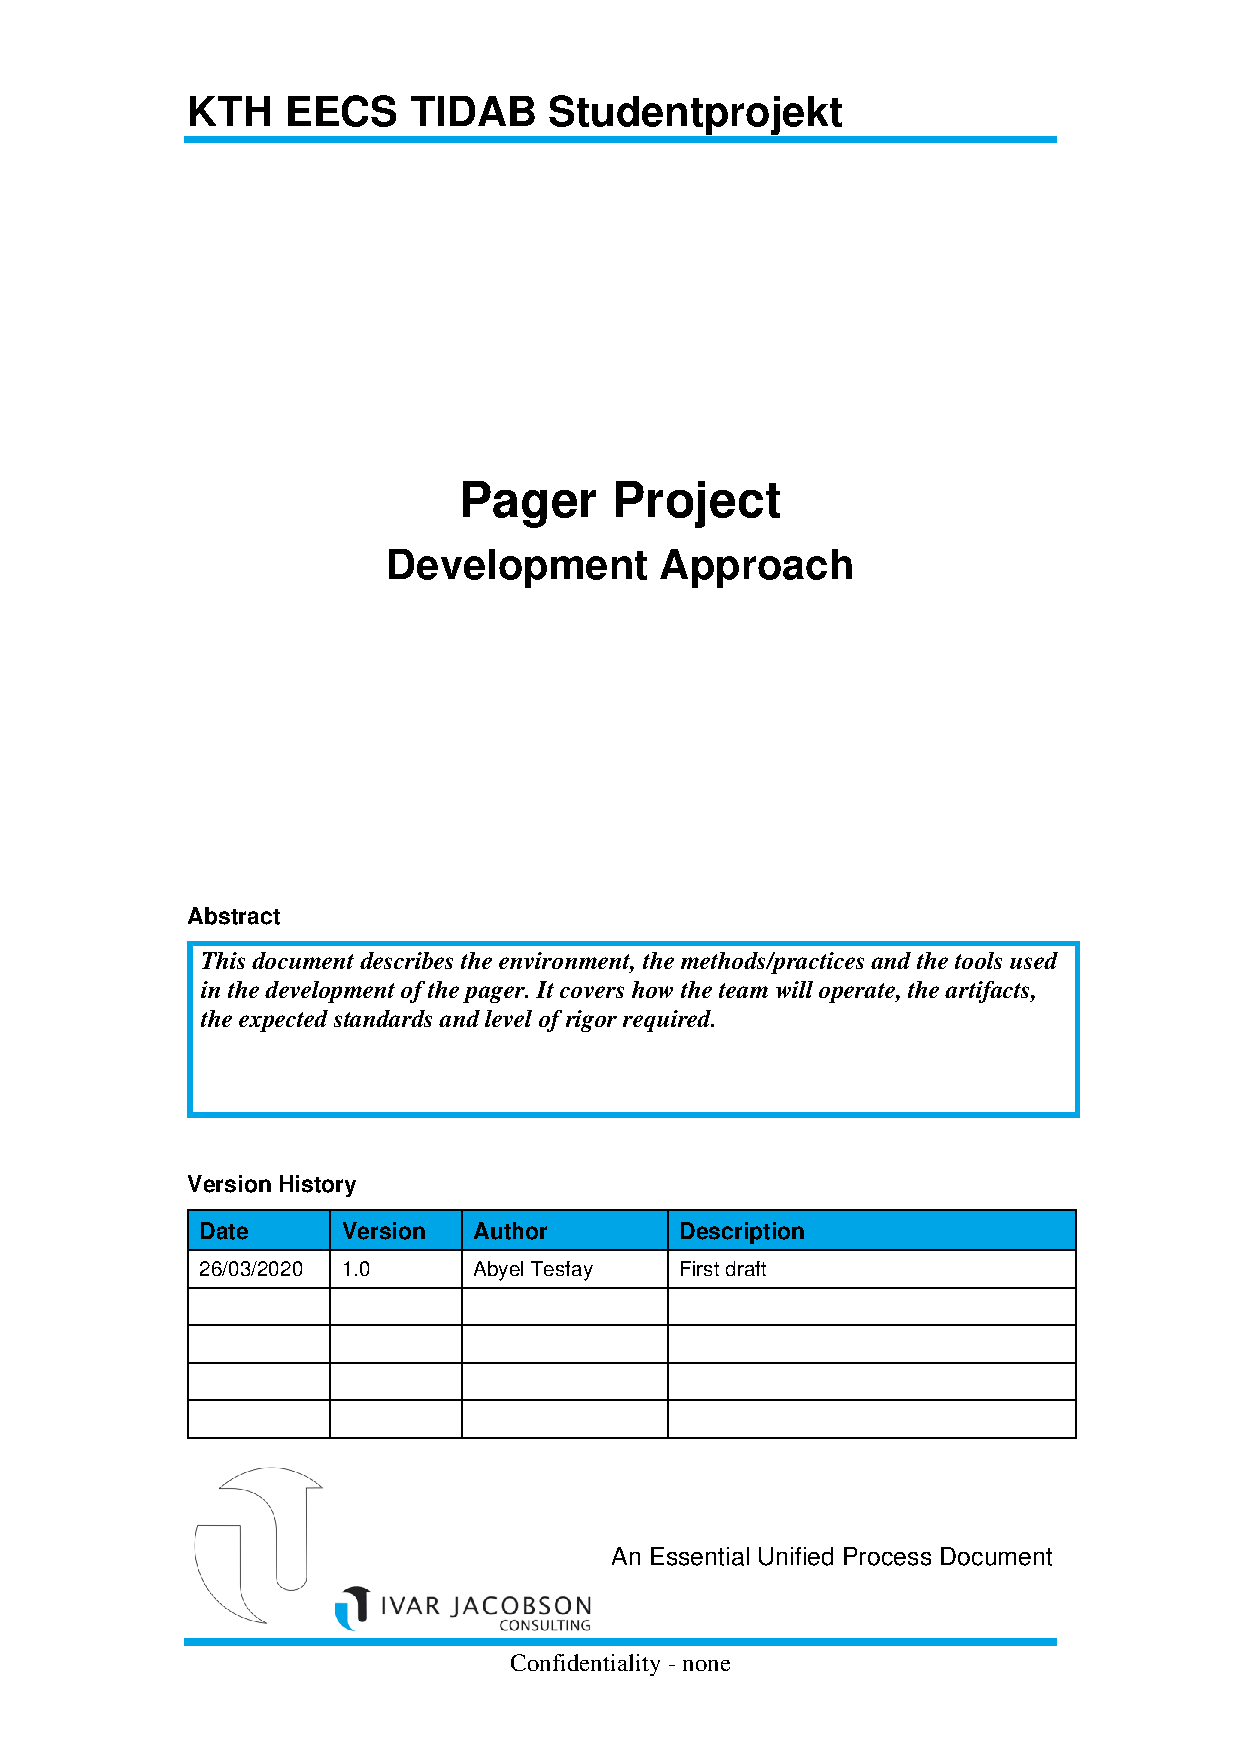
\includepdf[pages=-]{appendix/formell_at.pdf}
\end{appendix}

\begin{appendix}
    \begin{center}
        \large
        E:\\Formellt dokument: Alexander Johansson, testansvarig
    \end{center}

    \clearpage
    
\includepdf[pages=-]{appendix/formell_aj.pdf}
\end{appendix}

\begin{appendix}
    \begin{center}
        \large
        F:\\Tekniskt dokument: Adam Liliemark, cloud functions
    \end{center}

    \clearpage
    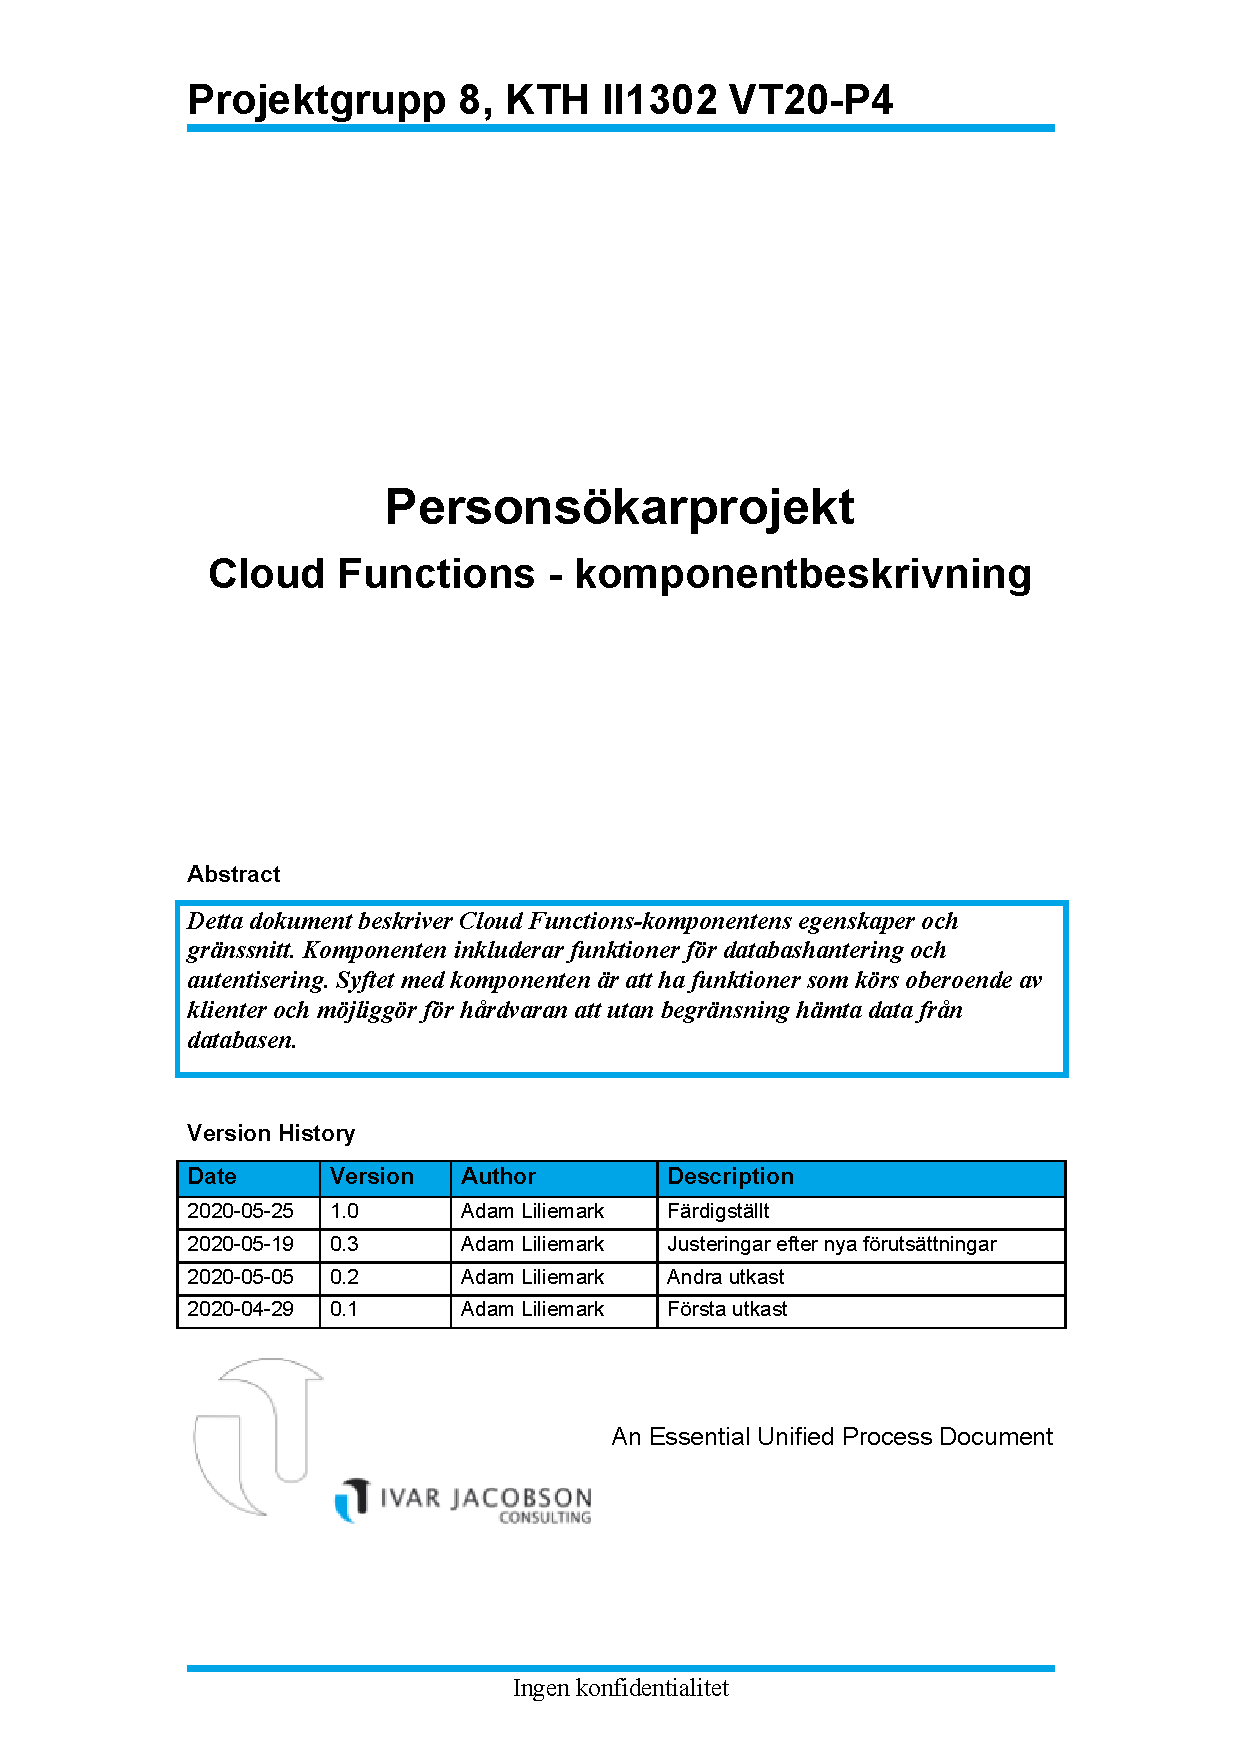
\includepdf[pages=-]{appendix/tekniskt_al.pdf}
\end{appendix}

\begin{appendix}
    \begin{center}
        \large
        G:\\Tekniskt dokument: Elias Johansson, wifi
    \end{center}

    \clearpage
    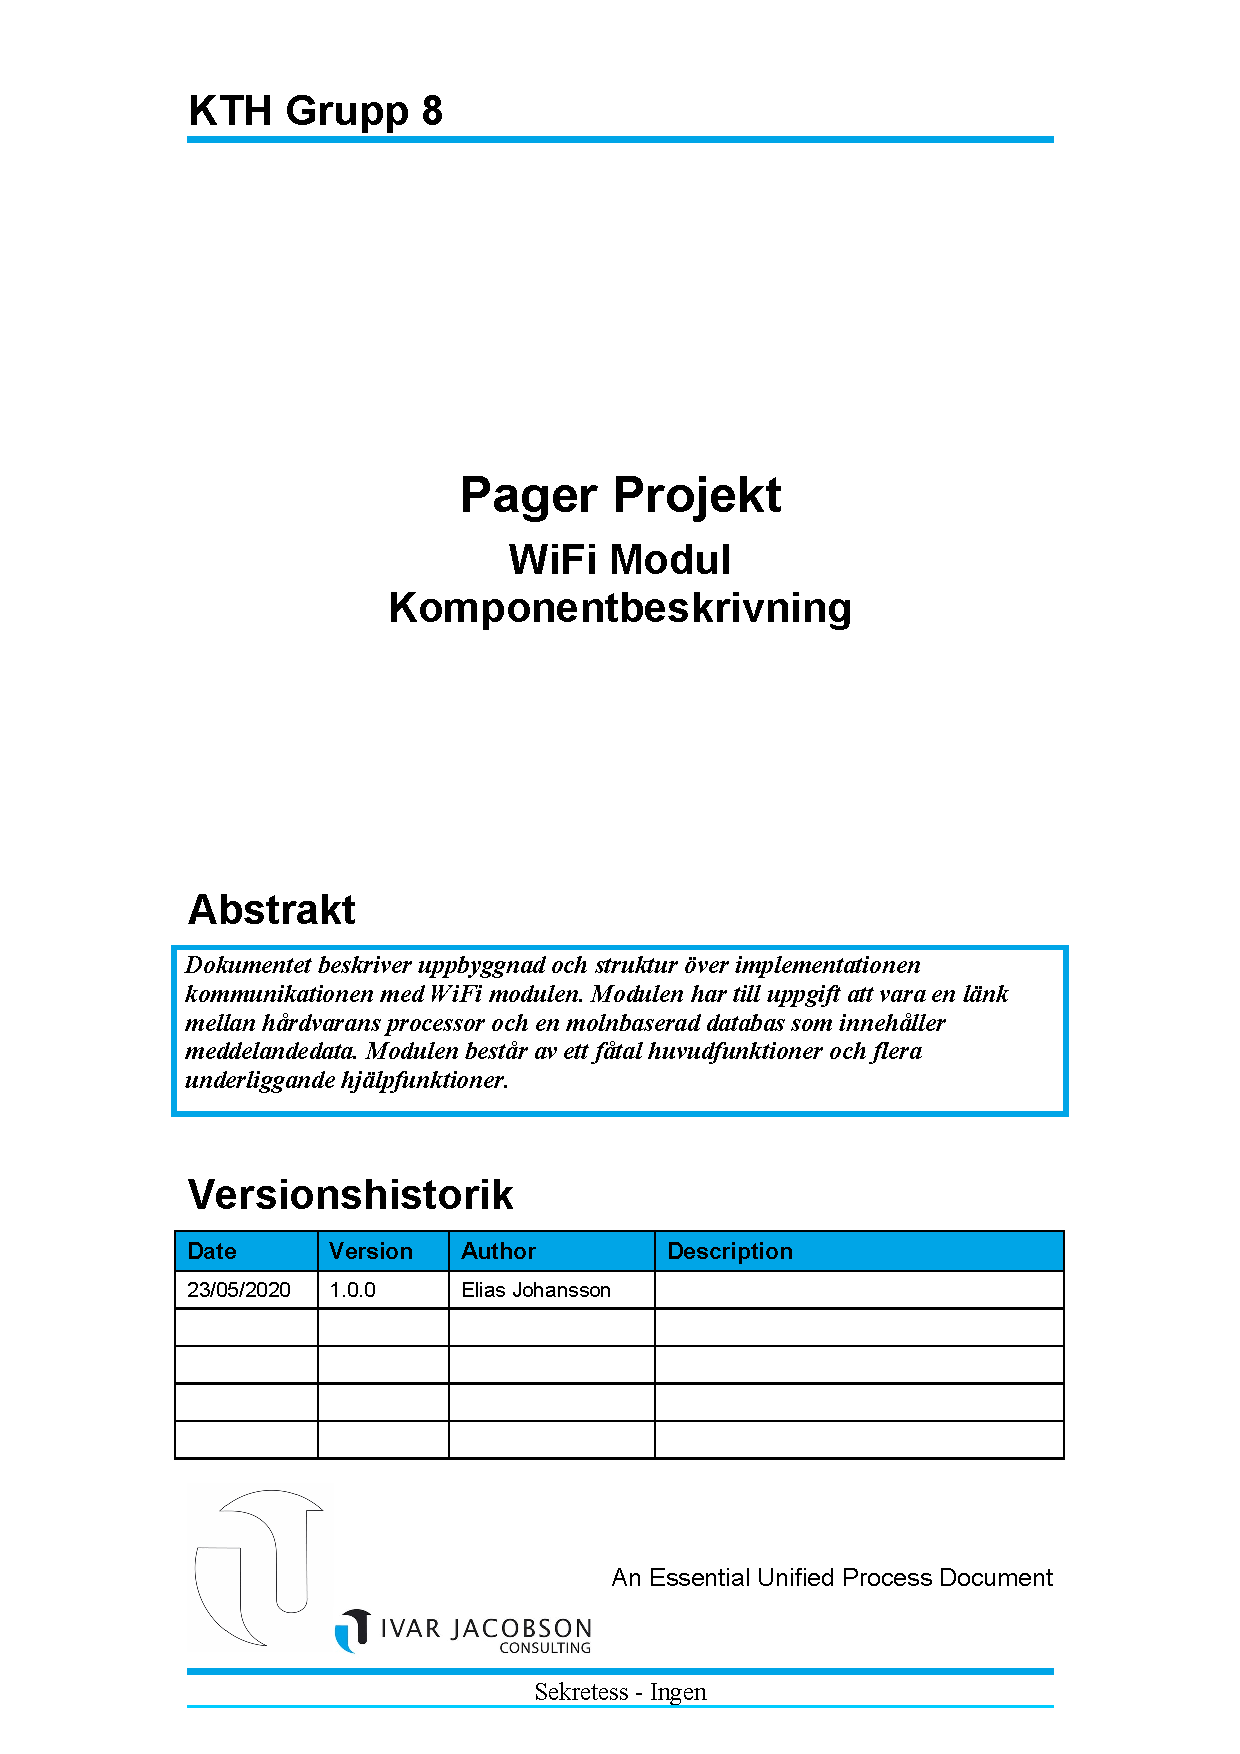
\includepdf[pages=-]{appendix/tekniskt_ej.pdf}
\end{appendix}

\begin{appendix}
    \begin{center}
        \large
        H:\\Tekniskt dokument: Mikael Andersson, knappsats
    \end{center}

    \clearpage
    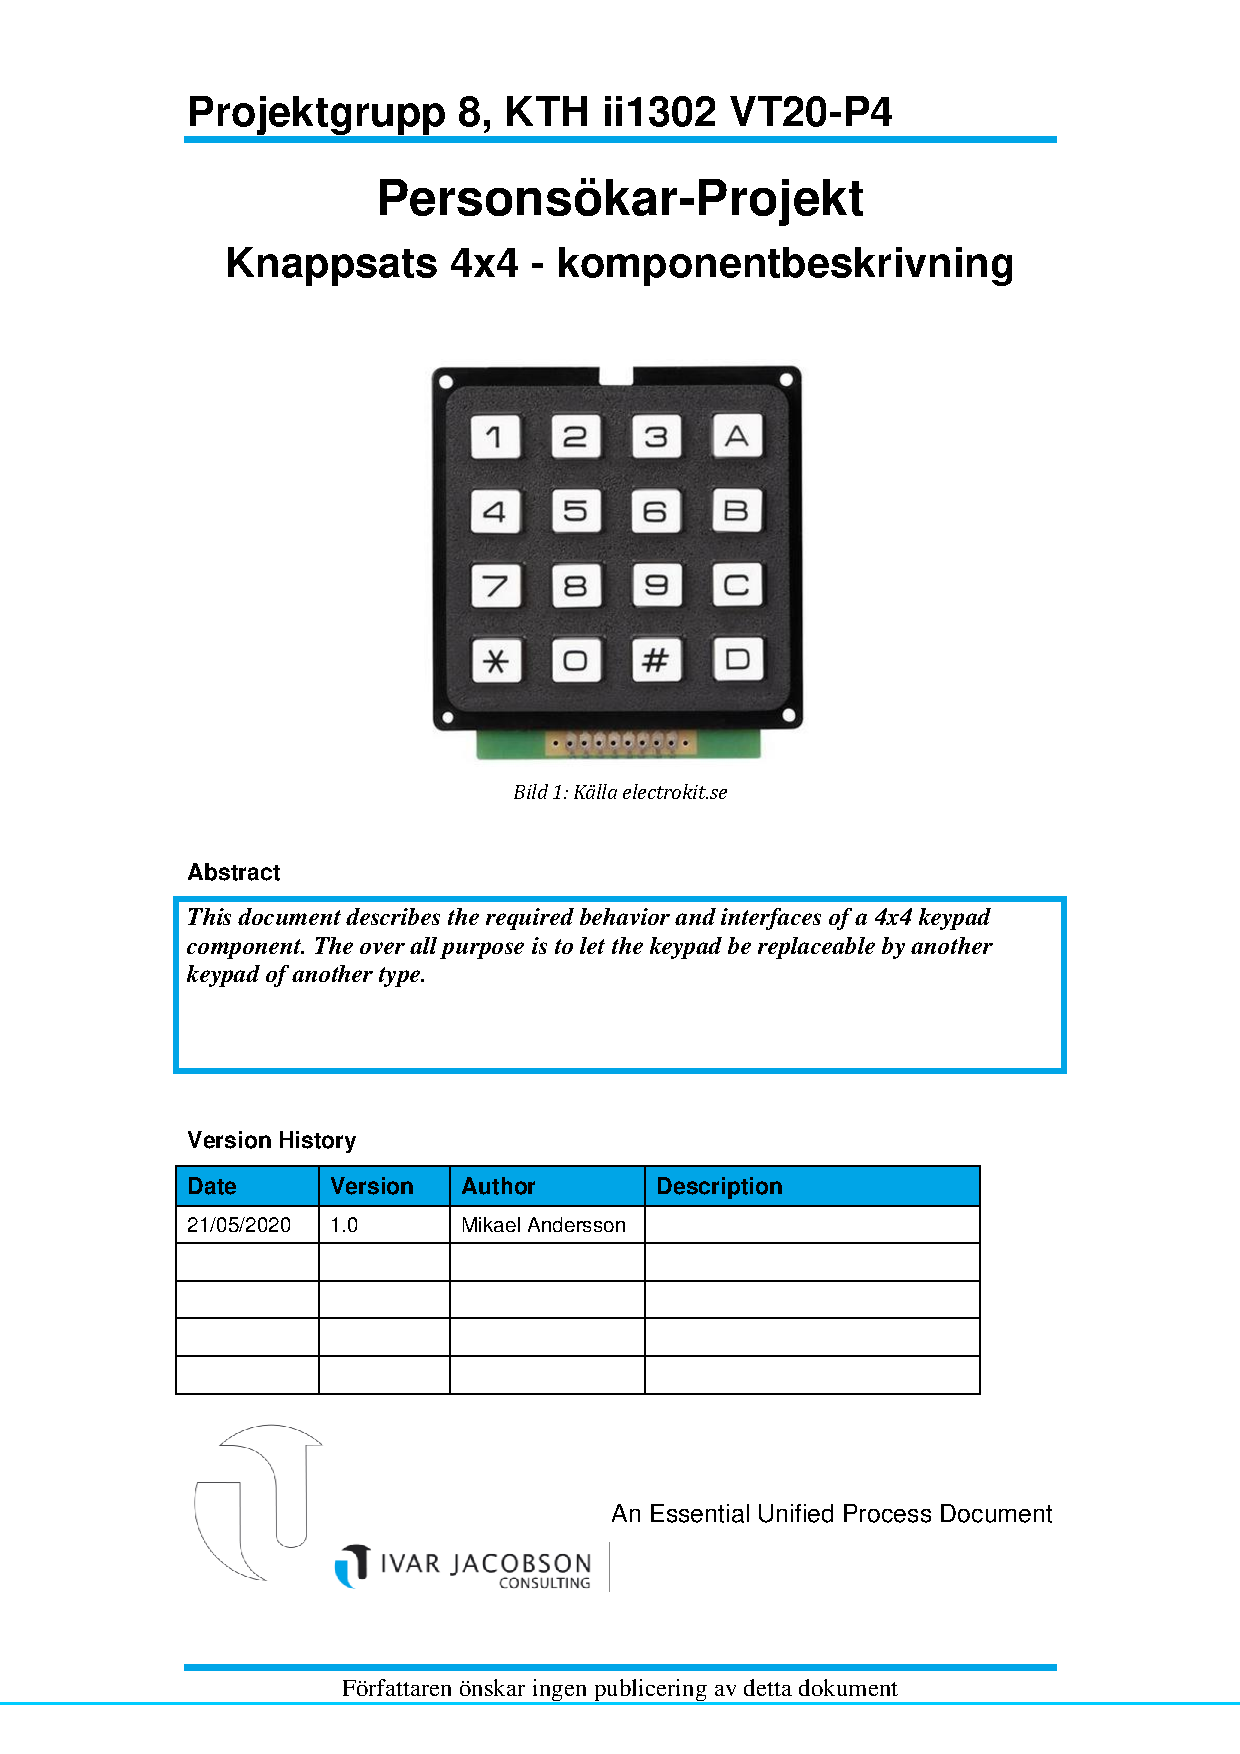
\includepdf[pages=-]{appendix/tekniskt_ma.pdf}
\end{appendix}

\begin{appendix}
    \begin{center}
        \large
        I:\\Tekniskt dokument: Abyel Tesfay, redux actions
    \end{center}

    \clearpage
    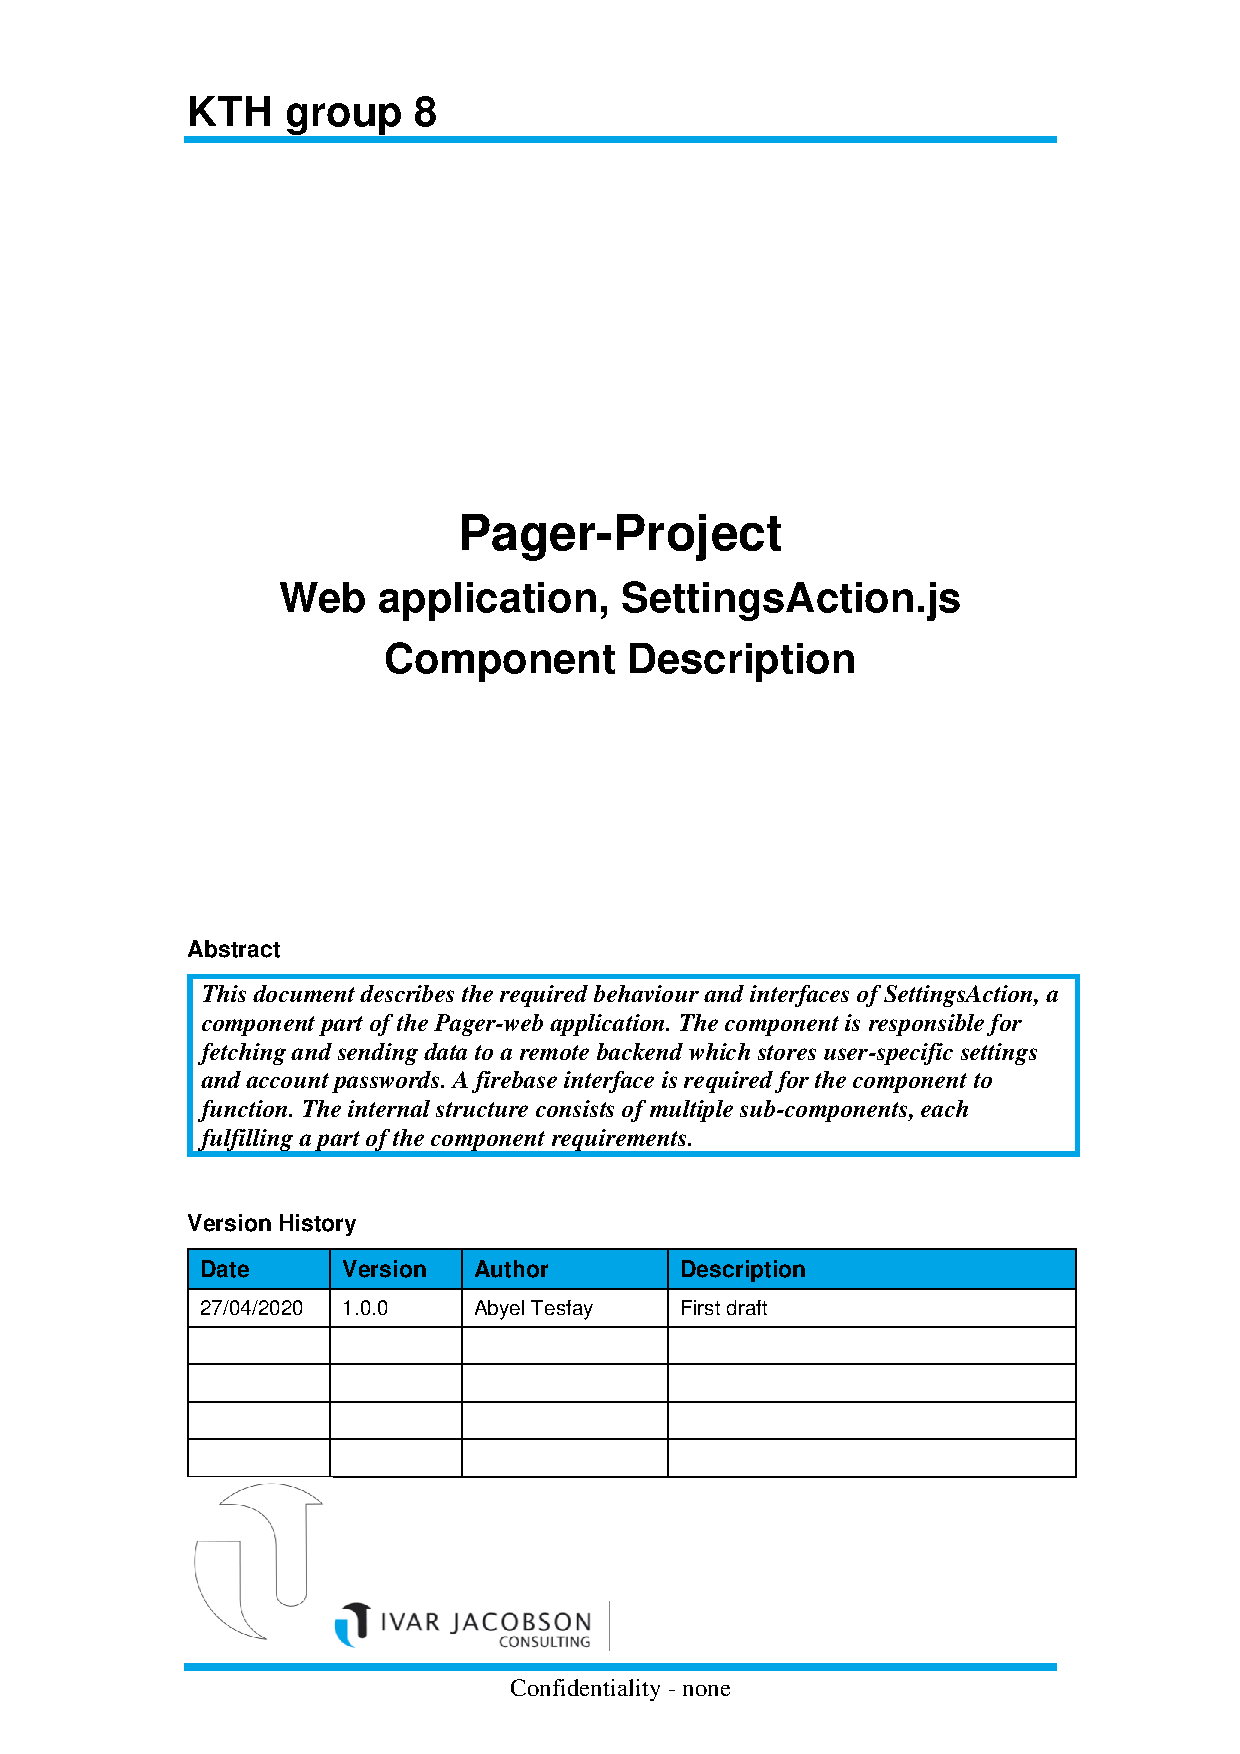
\includepdf[pages=-]{appendix/tekniskt_at.pdf}
\end{appendix}

\begin{appendix}
    \begin{center}
        \large
        J:\\Tekniskt dokument: Alexander Johansson, tester
    \end{center}

    \clearpage
    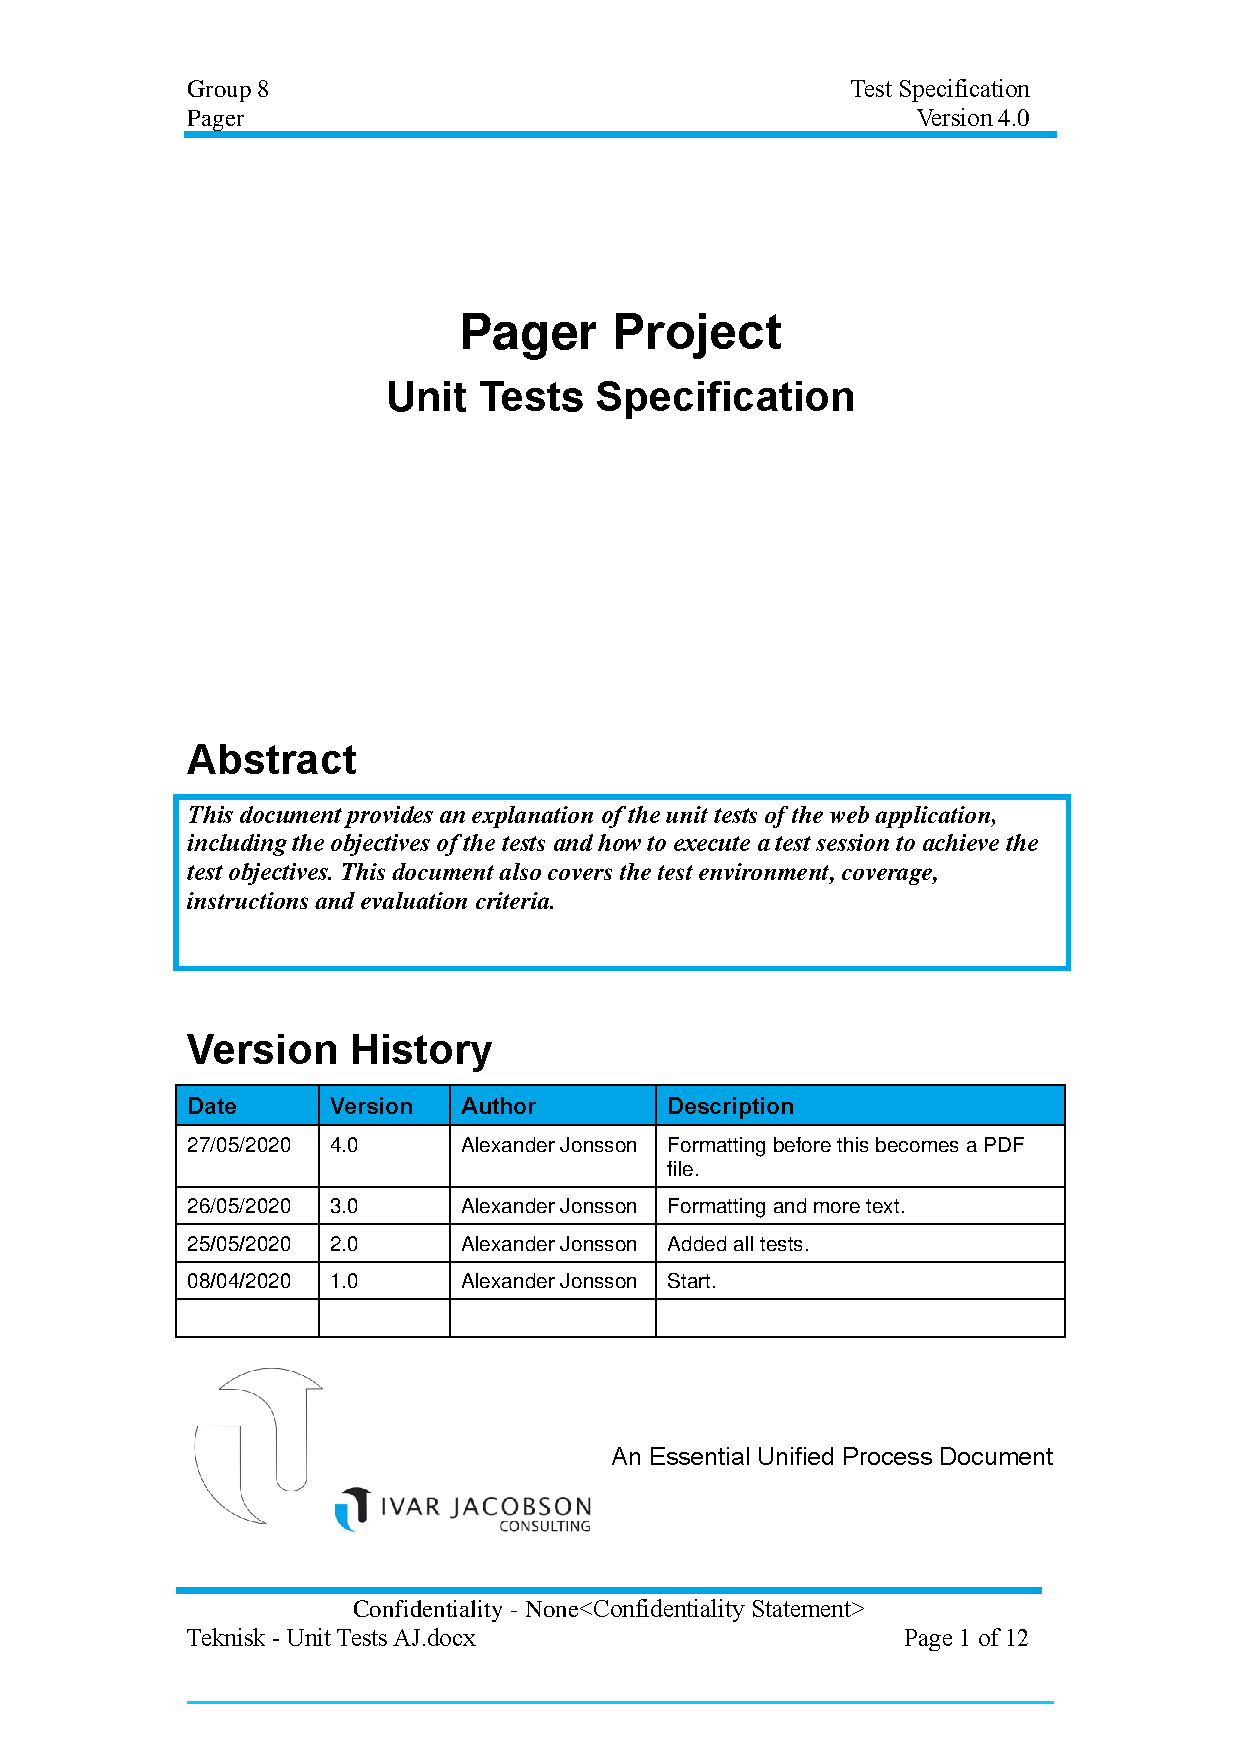
\includepdf[pages=-]{appendix/tekniskt_aj.pdf}
\end{appendix}

\begin{appendix}
    \begin{center}
        \large
        K:\\Kravspecifikation
    \end{center}

    \clearpage
    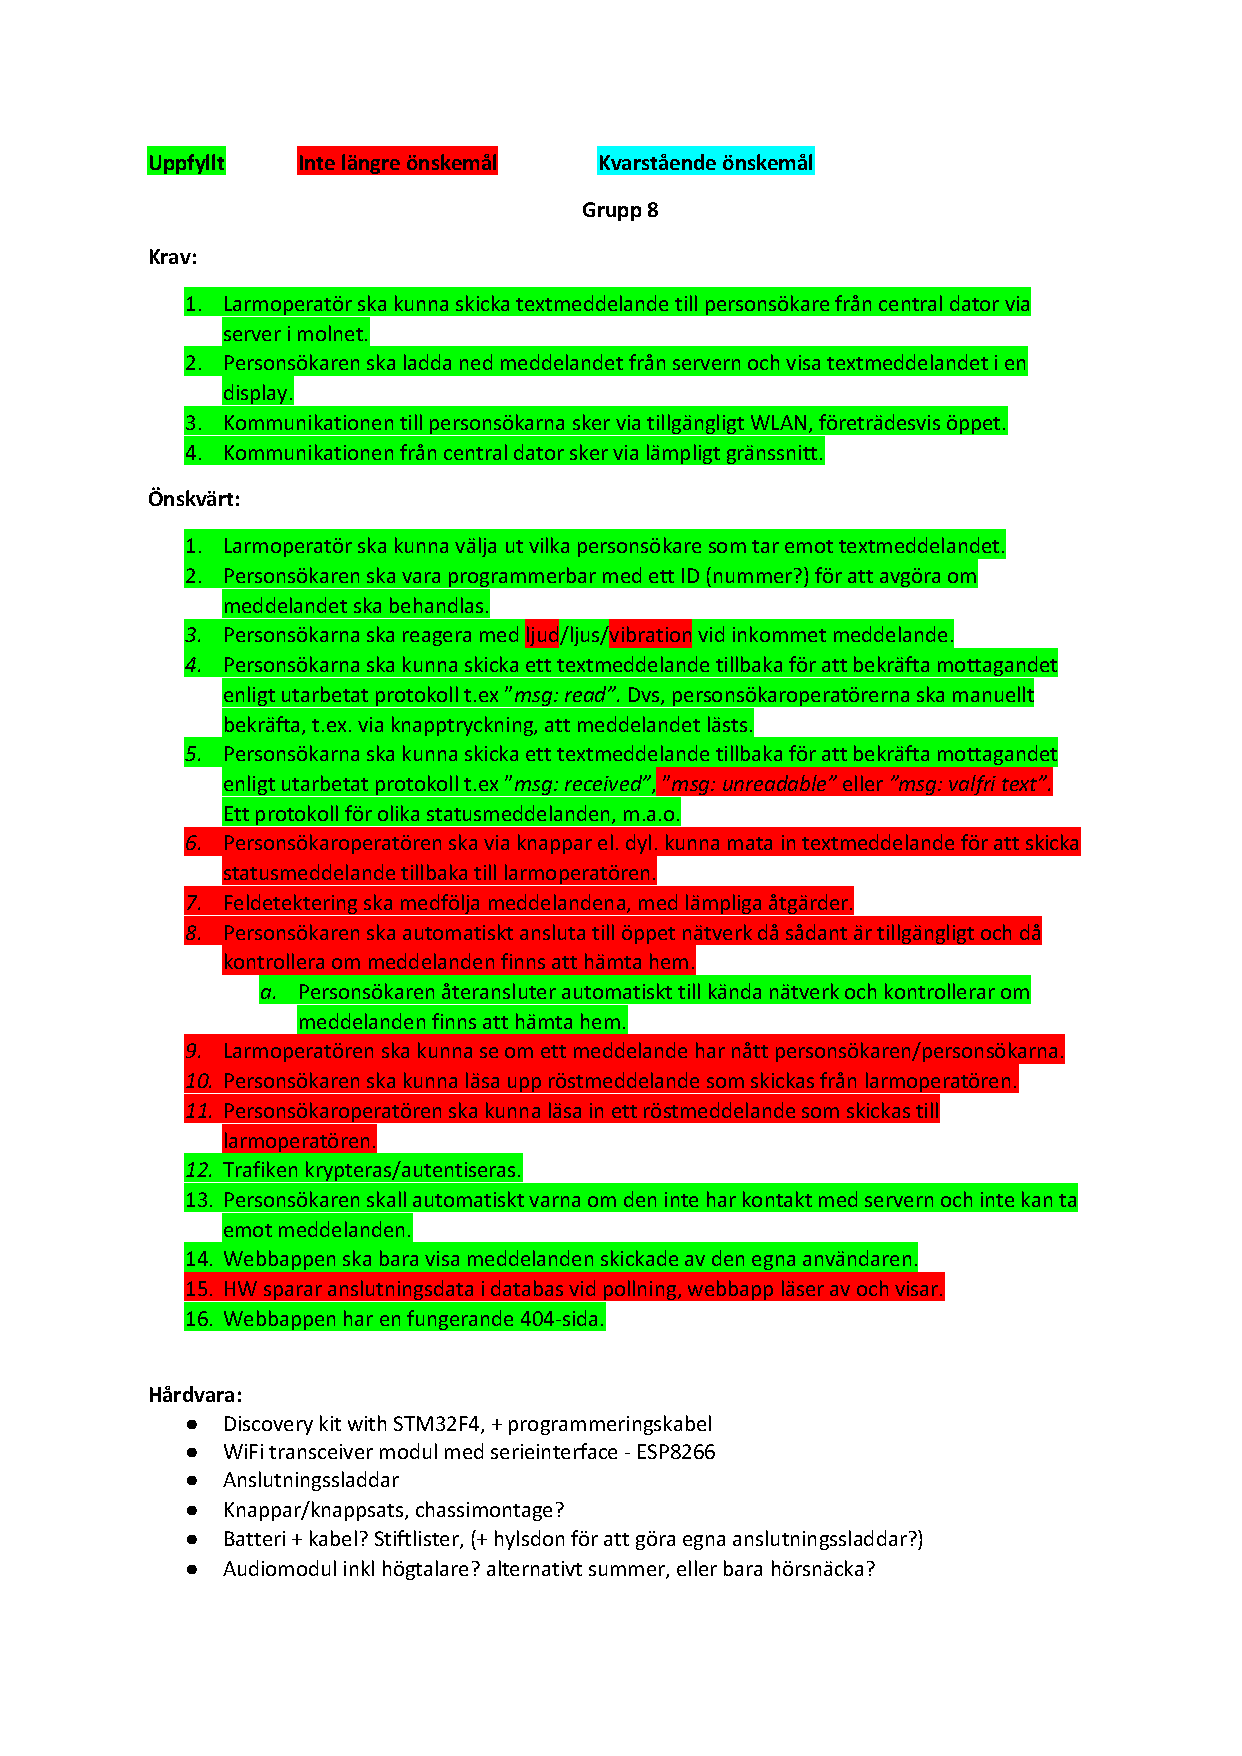
\includepdf[pages=-]{appendix/kravspec.pdf}
\end{appendix}

\begin{appendix}
    \begin{center}
        \large
        L:\\Projektdefinition
    \end{center}

    \clearpage
    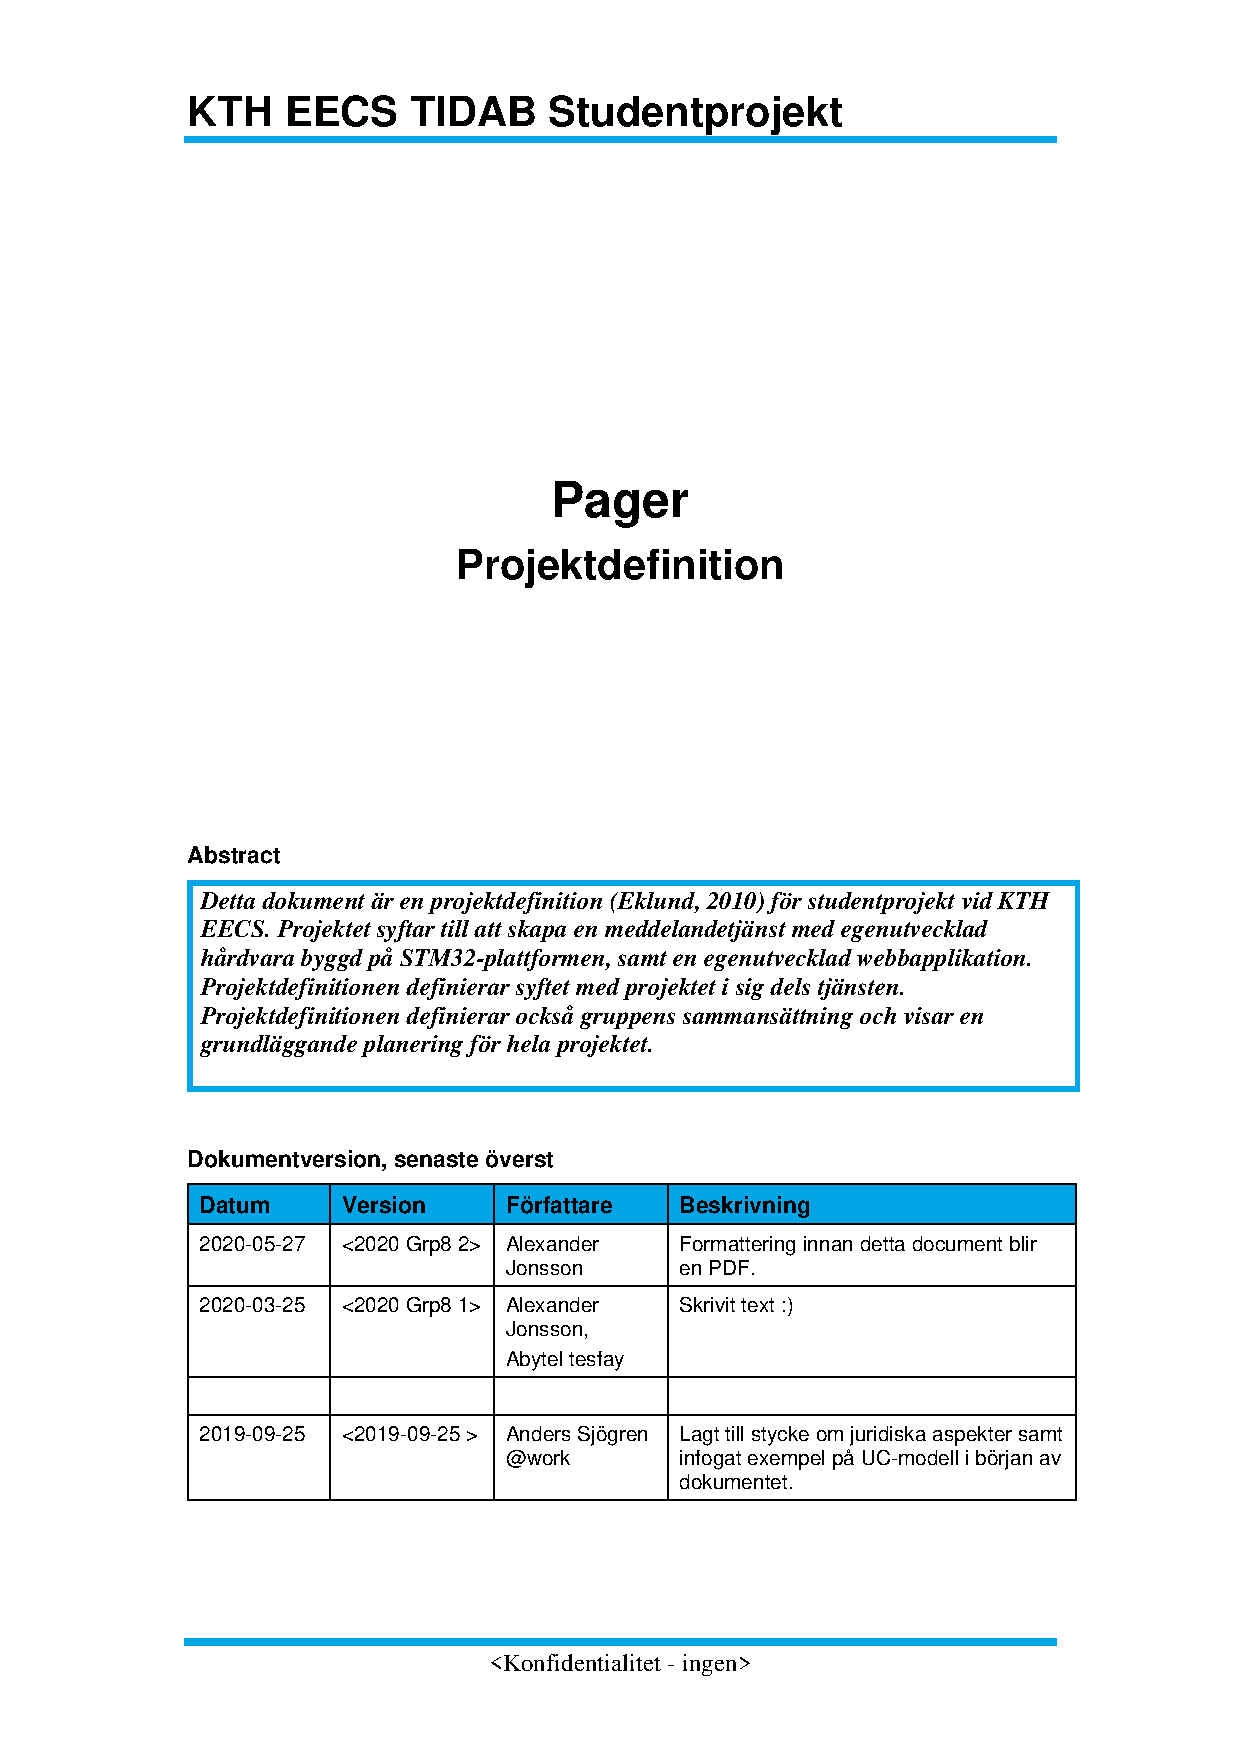
\includepdf[pages=-]{appendix/projektdef.pdf}
\end{appendix}

\end{document}
